%% (Master) Thesis template
% Template version used: v1.4
%
% Largely adapted from Adrian Nievergelt's template for the ADPS
% (lecture notes) project.


%% We use the memoir class because it offers a many easy to use features.
\documentclass[11pt,a4paper,titlepage]{memoir}

%% Packages
%% ========

% Lukas
\usepackage{subcaption}

%% LaTeX Font encoding -- DO NOT CHANGE
\usepackage[OT1]{fontenc}

%% Babel provides support for languages.  'english' uses British
%% English hyphenation and text snippets like "Figure" and
%% "Theorem". Use the option 'ngerman' if your document is in German.
%% Use 'american' for American English.  Note that if you change this,
%% the next LaTeX run may show spurious errors.  Simply run it again.
%% If they persist, remove the .aux file and try again.
\usepackage[american]{babel}

%% Input encoding 'utf8'. In some cases you might need 'utf8x' for
%% extra symbols. Not all editors, especially on Windows, are UTF-8
%% capable, so you may want to use 'latin1' instead.
\usepackage[utf8]{inputenc}

%% This changes default fonts for both text and math mode to use Herman Zapfs
%% excellent Palatino font.  Do not change this.
\usepackage[sc]{mathpazo}

%% The AMS-LaTeX extensions for mathematical typesetting.  Do not
%% remove.
\usepackage{amsmath,amssymb,amsfonts,mathrsfs}

%% NTheorem is a reimplementation of the AMS Theorem package. This
%% will allow us to typeset theorems like examples, proofs and
%% similar.  Do not remove.
%% NOTE: Must be loaded AFTER amsmath, or the \qed placement will
%% break
\usepackage[amsmath,thmmarks]{ntheorem}

%% LaTeX' own graphics handling
\usepackage{graphicx}

%% We unfortunately need this for the Rules chapter.  Remove it
%% afterwards; or at least NEVER use its underlining features.
\usepackage{soul}

%% This allows you to add .pdf files. It is used to add the
%% declaration of originality.
\usepackage{pdfpages}

%% Some more packages that you may want to use.  Have a look at the
%% file, and consult the package docs for each.
%% See the TeXed file for more explanations

%% [OPT] Multi-rowed cells in tabulars
%\usepackage{multirow}

%% [REC] Intelligent cross reference package. This allows for nice
%% combined references that include the reference and a hint to where
%% to look for it.
\usepackage{varioref}

%% [OPT] Easily changeable quotes with \enquote{Text}
%\usepackage[german=swiss]{csquotes}

%% [REC] Format dates and time depending on locale
\usepackage{datetime}

%% [OPT] Provides a \cancel{} command to stroke through mathematics.
%\usepackage{cancel}

%% [NEED] This allows for additional typesetting tools in mathmode.
%% See its excellent documentation.
\usepackage{mathtools}

%% [ADV] Conditional commands
%\usepackage{ifthen}

%% [OPT] Manual large braces or other delimiters.
%\usepackage{bigdelim, bigstrut}

%% [REC] Alternate vector arrows. Use the command \vv{} to get scaled
%% vector arrows.
\usepackage[h]{esvect}

%% [NEED] Some extensions to tabulars and array environments.
\usepackage{array}

%% [OPT] Postscript support via pstricks graphics package. Very
%% diverse applications.
%\usepackage{pstricks,pst-all}

%% [?] This seems to allow us to define some additional counters.
%\usepackage{etex}

%% [ADV] XY-Pic to typeset some matrix-style graphics
%\usepackage[all]{xy}

%% [OPT] This is needed to generate an index at the end of the
%% document.
%\usepackage{makeidx}

%% [OPT] Fancy package for source code listings.  The template text
%% needs it for some LaTeX snippets; remove/adapt the \lstset when you
%% remove the template content.
\usepackage{listings}
\lstset{language=TeX,basicstyle={\normalfont\ttfamily}}

%% [REC] Fancy character protrusion.  Must be loaded after all fonts.
\usepackage[activate]{pdfcprot}

%% [REC] Nicer tables.  Read the excellent documentation.
\usepackage{booktabs}

%% Lukas
\usepackage{amsmath}
\usepackage{longtable}
%\usepackage[dvipdfm]{graphicx}


%% Our layout configuration.  DO NOT CHANGE.
%% Memoir layout setup

%% NOTE: You are strongly advised not to change any of them unless you
%% know what you are doing.  These settings strongly interact in the
%% final look of the document.

% Dependencies
\usepackage{0general/ETHlogo}

% Turn extra space before chapter headings off.
\setlength{\beforechapskip}{0pt}

\nonzeroparskip
\parindent=0pt
\defaultlists

% Chapter style redefinition
\makeatletter

\if@twoside
  \pagestyle{Ruled}
  \copypagestyle{chapter}{Ruled}
\else
  \pagestyle{ruled}
  \copypagestyle{chapter}{ruled}
\fi
\makeoddhead{chapter}{}{}{}
\makeevenhead{chapter}{}{}{}
\makeheadrule{chapter}{\textwidth}{0pt}
\copypagestyle{abstract}{empty}

\makechapterstyle{bianchimod}{%
  \chapterstyle{default}
  \renewcommand*{\chapnamefont}{\normalfont\Large\sffamily}
  \renewcommand*{\chapnumfont}{\normalfont\Large\sffamily}
  \renewcommand*{\printchaptername}{%
    \chapnamefont\centering\@chapapp}
  \renewcommand*{\printchapternum}{\chapnumfont {\thechapter}}
  \renewcommand*{\chaptitlefont}{\normalfont\huge\sffamily}
  \renewcommand*{\printchaptertitle}[1]{%
    \hrule\vskip\onelineskip \centering \chaptitlefont\textbf{\vphantom{gyM}##1}\par}
  \renewcommand*{\afterchaptertitle}{\vskip\onelineskip \hrule\vskip
    \afterchapskip}
  \renewcommand*{\printchapternonum}{%
    \vphantom{\chapnumfont {9}}\afterchapternum}}

% Use the newly defined style
\chapterstyle{bianchimod}

\setsecheadstyle{\Large\bfseries\sffamily}
\setsubsecheadstyle{\large\bfseries\sffamily}
\setsubsubsecheadstyle{\bfseries\sffamily}
\setparaheadstyle{\normalsize\bfseries\sffamily}
\setsubparaheadstyle{\normalsize\itshape\sffamily}
\setsubparaindent{0pt}

% Set captions to a more separated style for clearness
\captionnamefont{\sffamily\bfseries\footnotesize}
\captiontitlefont{\sffamily\footnotesize}
\setlength{\intextsep}{16pt}
\setlength{\belowcaptionskip}{1pt}

% subcaptions by Lukas
\captionsetup[sub]{font=footnotesize, labelfont={sf,bf}, textfont=sf}
\captionsetup{font=footnotesize, labelfont={sf,bf}, textfont=sf}


% Set section and TOC numbering depth to subsection
\setsecnumdepth{subsection}
\settocdepth{subsection}

%% Titlepage adjustments
\pretitle{\vspace{0pt plus 0.7fill}\begin{center}\HUGE\sffamily\bfseries}
\posttitle{\end{center}\par}
\preauthor{\par\begin{center}\let\and\\\Large\sffamily}
\postauthor{\end{center}}
\predate{\par\begin{center}\Large\sffamily}
\postdate{\end{center}}

\def\@advisors{}
\newcommand{\advisors}[1]{\def\@advisors{#1}}
\def\@department{}
\newcommand{\department}[1]{\def\@department{#1}}
\def\@thesistype{}
\newcommand{\thesistype}[1]{\def\@thesistype{#1}}

\renewcommand{\maketitlehooka}{\noindent\ETHlogo[2in]}

\renewcommand{\maketitlehookb}{\vspace{1in}%
  \par\begin{center}\Large\sffamily\@thesistype\end{center}}

\renewcommand{\maketitlehookd}{%
  \vfill\par
  \begin{flushright}
    \sffamily
    \@advisors\par
    \@department, ETH Z\"urich
  \end{flushright}
}

\checkandfixthelayout

\setlength{\droptitle}{-48pt}

\makeatother

% This defines how theorems should look. Best leave as is.
\theoremstyle{plain}
\setlength\theorempostskipamount{0pt}

%%% Local Variables:
%%% mode: latex
%%% TeX-master: "thesis"
%%% End:


%% Theorem environments.  You will have to adapt this for a German
%% thesis.
%% Theorem-like environments

%% This can be changed according to language. You can comment out the ones you
%% don't need.

\numberwithin{equation}{chapter}

%% German theorems
%\newtheorem{satz}{Satz}[chapter]
%\newtheorem{beispiel}[satz]{Beispiel}
%\newtheorem{bemerkung}[satz]{Bemerkung}
%\newtheorem{korrolar}[satz]{Korrolar}
%\newtheorem{definition}[satz]{Definition}
%\newtheorem{lemma}[satz]{Lemma}
%\newtheorem{proposition}[satz]{Proposition}

%% English variants
\newtheorem{theorem}{Theorem}[chapter]
\newtheorem{example}[theorem]{Example}
\newtheorem{remark}[theorem]{Remark}
\newtheorem{corollary}[theorem]{Corollary}
\newtheorem{definition}[theorem]{Definition}
\newtheorem{lemma}[theorem]{Lemma}
\newtheorem{proposition}[theorem]{Proposition}

%% Proof environment with a small square as a "qed" symbol
\theoremstyle{nonumberplain}
\theorembodyfont{\normalfont}
\theoremsymbol{\ensuremath{\square}}
\newtheorem{proof}{Proof}
%\newtheorem{beweis}{Beweis}


%% Helpful macros.
%% Custom commands
%% ===============

%% Special characters for number sets, e.g. real or complex numbers.
\newcommand{\C}{\mathbb{C}}
\newcommand{\K}{\mathbb{K}}
\newcommand{\N}{\mathbb{N}}
\newcommand{\Q}{\mathbb{Q}}
\newcommand{\R}{\mathbb{R}}
\newcommand{\Z}{\mathbb{Z}}
\newcommand{\X}{\mathbb{X}}

%% Fixed/scaling delimiter examples (see mathtools documentation)
\DeclarePairedDelimiter\abs{\lvert}{\rvert}
\DeclarePairedDelimiter\norm{\lVert}{\rVert}

%% Use the alternative epsilon per default and define the old one as \oldepsilon
\let\oldepsilon\epsilon
\renewcommand{\epsilon}{\ensuremath\varepsilon}

%% Also set the alternate phi as default.
\let\oldphi\phi
\renewcommand{\phi}{\ensuremath{\varphi}}


%% Make document internal hyperlinks wherever possible. (TOC, references)
%% This MUST be loaded after varioref, which is loaded in 'extrapackages'
%% above.  We just load it last to be safe.
\usepackage[linkcolor=black,colorlinks=true,citecolor=black,filecolor=black]{hyperref}


%% Document information
%% ====================

\title{Hierarchical Paragraph Vectors}
\author{Lukas Elmer}
\thesistype{Master Thesis}
\advisors{Advisors: Prof.\ Dr.\ Thomas Hofmann, Dr.\ Carsten Eickhoff}
\department{Department of Computer Science}
\date{September 8, 2015}

\begin{document}

\frontmatter

%% Title page is autogenerated from document information above.  DO
%% NOT CHANGE.
\begin{titlingpage}
  \calccentering{\unitlength}
  \begin{adjustwidth*}{\unitlength-24pt}{-\unitlength-24pt}
    \maketitle
  \end{adjustwidth*}
\end{titlingpage}

%% The abstract of your thesis.  Edit the file as needed.
\begin{abstract}
	Most standard machine learning algorithms require fixed-length, low-dimensional vectors to perform well. However, when working with text, such representations are difficult to obtain. In 2014, Le and Mikolov presented a novel method for generating so-called word embeddings \cite{Mikolov2013}. Their work represents the foundation for this master thesis.
	
	The main goal of this thesis is to extend and generalize the word embedding model to a hierarchical paragraph vector model. This means that different parts of the vector represent different contexts which are shared among sibling structures originating from the same parent text block. For example, the first part of the vector can be used to describe the document, the second part to describe the chapter, the third part to describe the paragraph and the last part to describe the individual sentence.
	
	In this thesis, we propose \emph{Hierarchical Paragraph Vectors}, which exploit hierarchical document structures. When applying this novel method to sentiment analysis tasks, empirical results show that it can increase the quality of the word embeddings at the cost of greater execution overhead.
	
	%In this thesis, we propose \emph{Hierarchical Paragraph Vectors}, which exploits hierarchical information to improve the quality of the word embeddings. When applying this novel method to sentiment analysis tasks, empirical results show that it can increase the quality of the word embeddings at the cost of greater overhead.
	%The main goal of this thesis is to extend and generalize the word embedding model of \cite{Mikolov2013} to a hierarchical paragraph vector model. The introduced paragraph vector model by Le and Mikolov shares one paragraph vector within a block of text.
	%The main goal of this thesis is to extend and generalize the word embedding model of \cite{Mikolov2013}. The introduced paragraph vector by Le and Mikolov represents a block of text by a single dedicated vector, which is shared within a block of text.
	%This master thesis is based on distributed representations of sentences and documents \cite{Mikolov2013}. Currently, the paragraph vector model represents a block of text (for example a document) by a single dedicated vector. As a consequence, individual sub-blocks within a block of text do not share any information among each other.
	%The main goal of this master thesis is to extend and generalize the word embedding model to a hierarchical paragraph vector model. This means that different parts of the vector represent different contexts, and are shared among siblings originating from the same parent text block. For example, the first part of the vector can be used to describe the document, the second part to describe the chapter, the third part to describe the paragraph and the last part to describe the sentence.
	%[peek into results and experiments]
\end{abstract}

\clearpage

\renewcommand{\abstractname}{Acknowledgements}

\begin{abstract}
I would like to thank Dr. Carsten Eickhoff for his continuous support, insightful and straightforward advice, positive criticism, proofreading, and the supervision of my master thesis. It has been a pleasure working with him.

Additionally, I would like to thank Prof. Dr. Thomas Hofmann for giving me the opportunity to investigating the highly interesting topics of NLP and word embeddings, and for his valuable feedback.

Furthermore, I would like to thank everyone who supported me during my studies, especially my family, my business partners and colleagues\footnote{\url{https://www.renuo.ch}}, for their support, understanding, and positive attitude.

Finally, I would like to thank Marion for her continuous positive attitude, proofreading, and for being by my side.
\end{abstract}


%% TOC with the proper setup, do not change.
\cleartorecto
\tableofcontents
\mainmatter

%% Your real content!
\chapter{Introduction}

Words are the building blocks of natural language. Words are categorized into word classes (for example verbs, nouns, adjectives) and any given grammar only allows certain combinations and word orders to form valid sentences. The meaning of these words is manifold, and naturally some words are more similar to each other than they are to others. Consider for example the three words ``interesting'', ``fascinating'' and ``bottle''. In this case, the first two words are more similar to each other.
Hence, the idea to represent words in a way that captures these similarities, is natural. One way of achieving this is the use of semantically informed vector representations, so-called word embeddings.

Finding suitable word embeddings is a challenging and interesting task. The objective is to find a low-dimensional vector for each word and/or phrase in the vocabulary. When done correctly, these word embeddings have been shown to be useful to help solving difficult Natural Language Processing (NLP) problems, including machine translation~\cite{Mikolov2013b, Wolf2013}, sentence completion~\cite{Mikolov2013a}, sentiment analysis~\cite{Hong}, and topic modeling~\cite{Jameel2013}.

Recent advancements~\cite{Mikolov2013a, Mikolov2013} allow finding high-quality low-dimensional word embeddings, while the processing speed is increased substantially due to many optimizations and/or approximations. Furthermore, reliable and fast implementations have been developed and released, one of them being Gensim~\cite{rehurek_lrec}. Therefore, training a word embedding model is now feasible within minutes or hours, while it took days or months before~\cite{Mikolov2013}.

For many applications, the data is formatted in a hierarchical structure, as can be observed in Figures~\ref{fig:1:hierarchies-wikipedia-syntax},~\ref{fig:1:hierarchies-categories} and~\ref{fig:1:hierarchies-sports}. Therefore, it is compelling to try exploiting these hierarchies to improve the quality of the word embeddings and/or to reduce the learning time while maintaining the word vector quality. To our best knowledge, this concept has not been investigated profoundly yet, using the recent advancements in~\cite{Mikolov2013}, although there have been motions towards this direction already~\cite{Fu2014}.

%todo tbd carsten: maybe include one more paragraph on why we think this should help and what it should achieve.

\begin{figure}
	\centering
	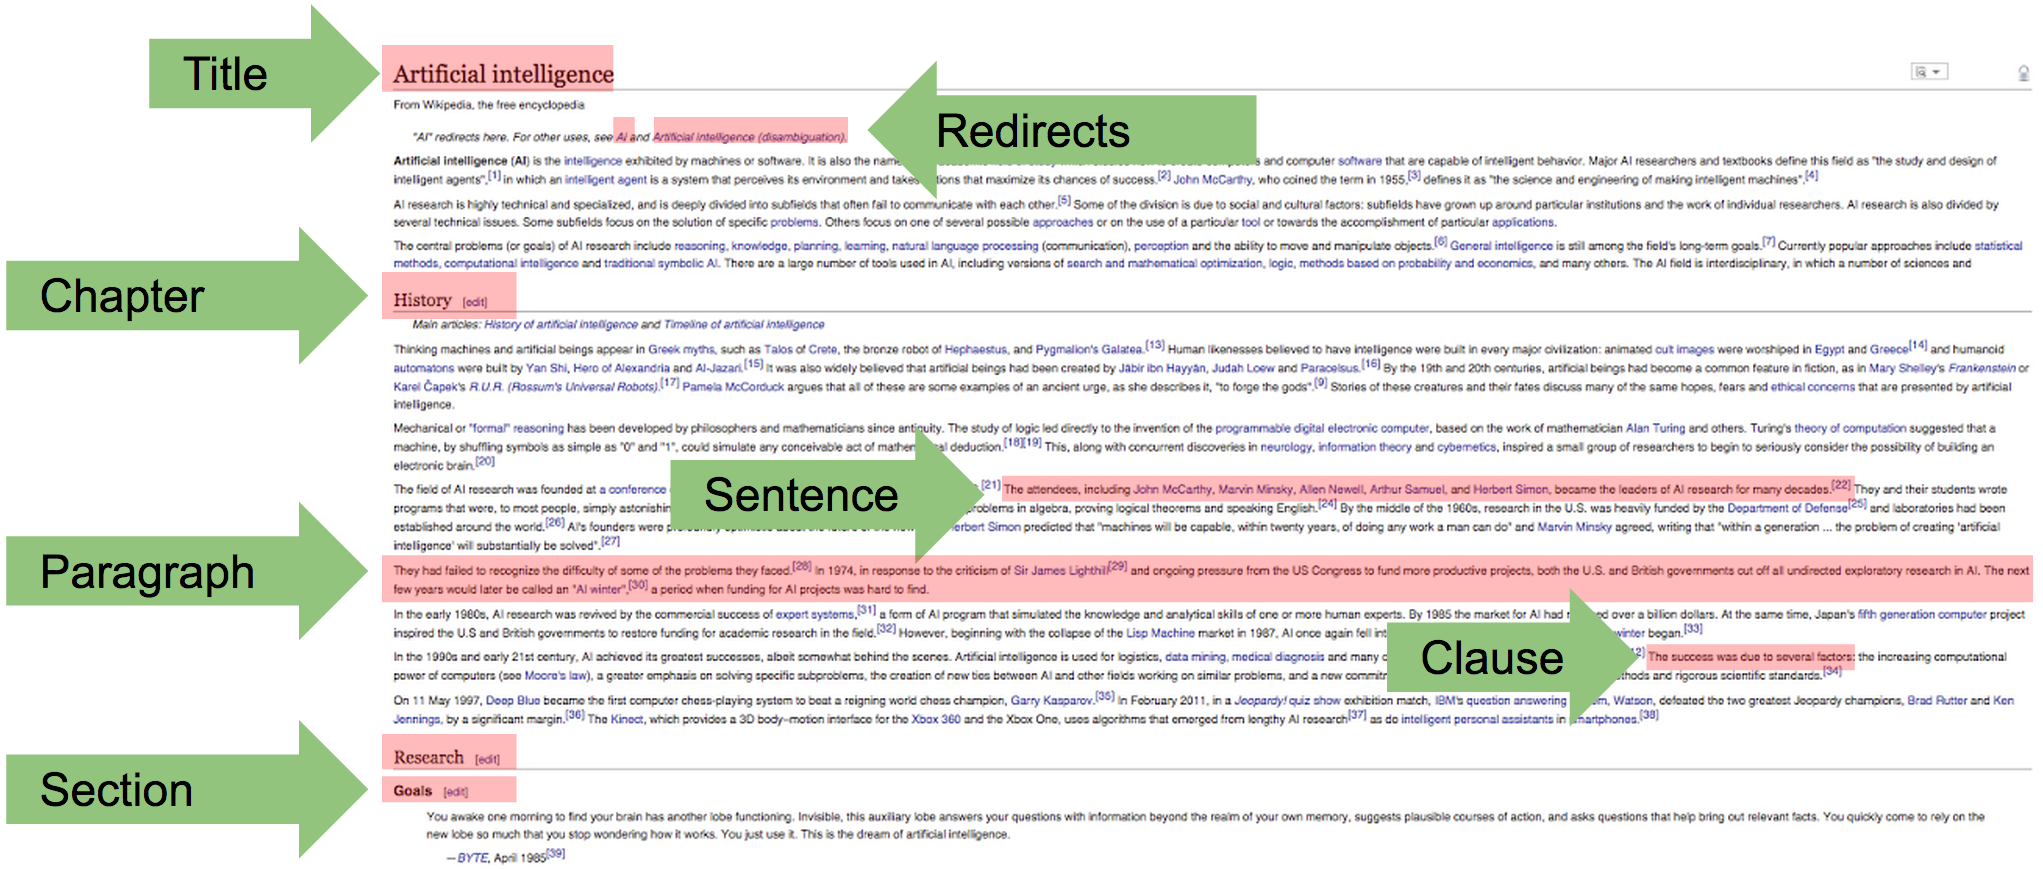
\includegraphics[width=1.0\textwidth]{1introduction/hierarchies-wikipedia-syntax.png}
	\caption[Caption for LOF]{The Wikipedia article about artificial intelligence is segmented into semantic and syntactic hierarchies (for example title, chapter, section, paragraph, sentence, clause).\footnotemark}
	\label{fig:1:hierarchies-wikipedia-syntax}
\end{figure}

\footnotetext{Source: \url{https://en.wikipedia.org/wiki/Artificial_intelligence}}

\begin{figure}
	\centering
	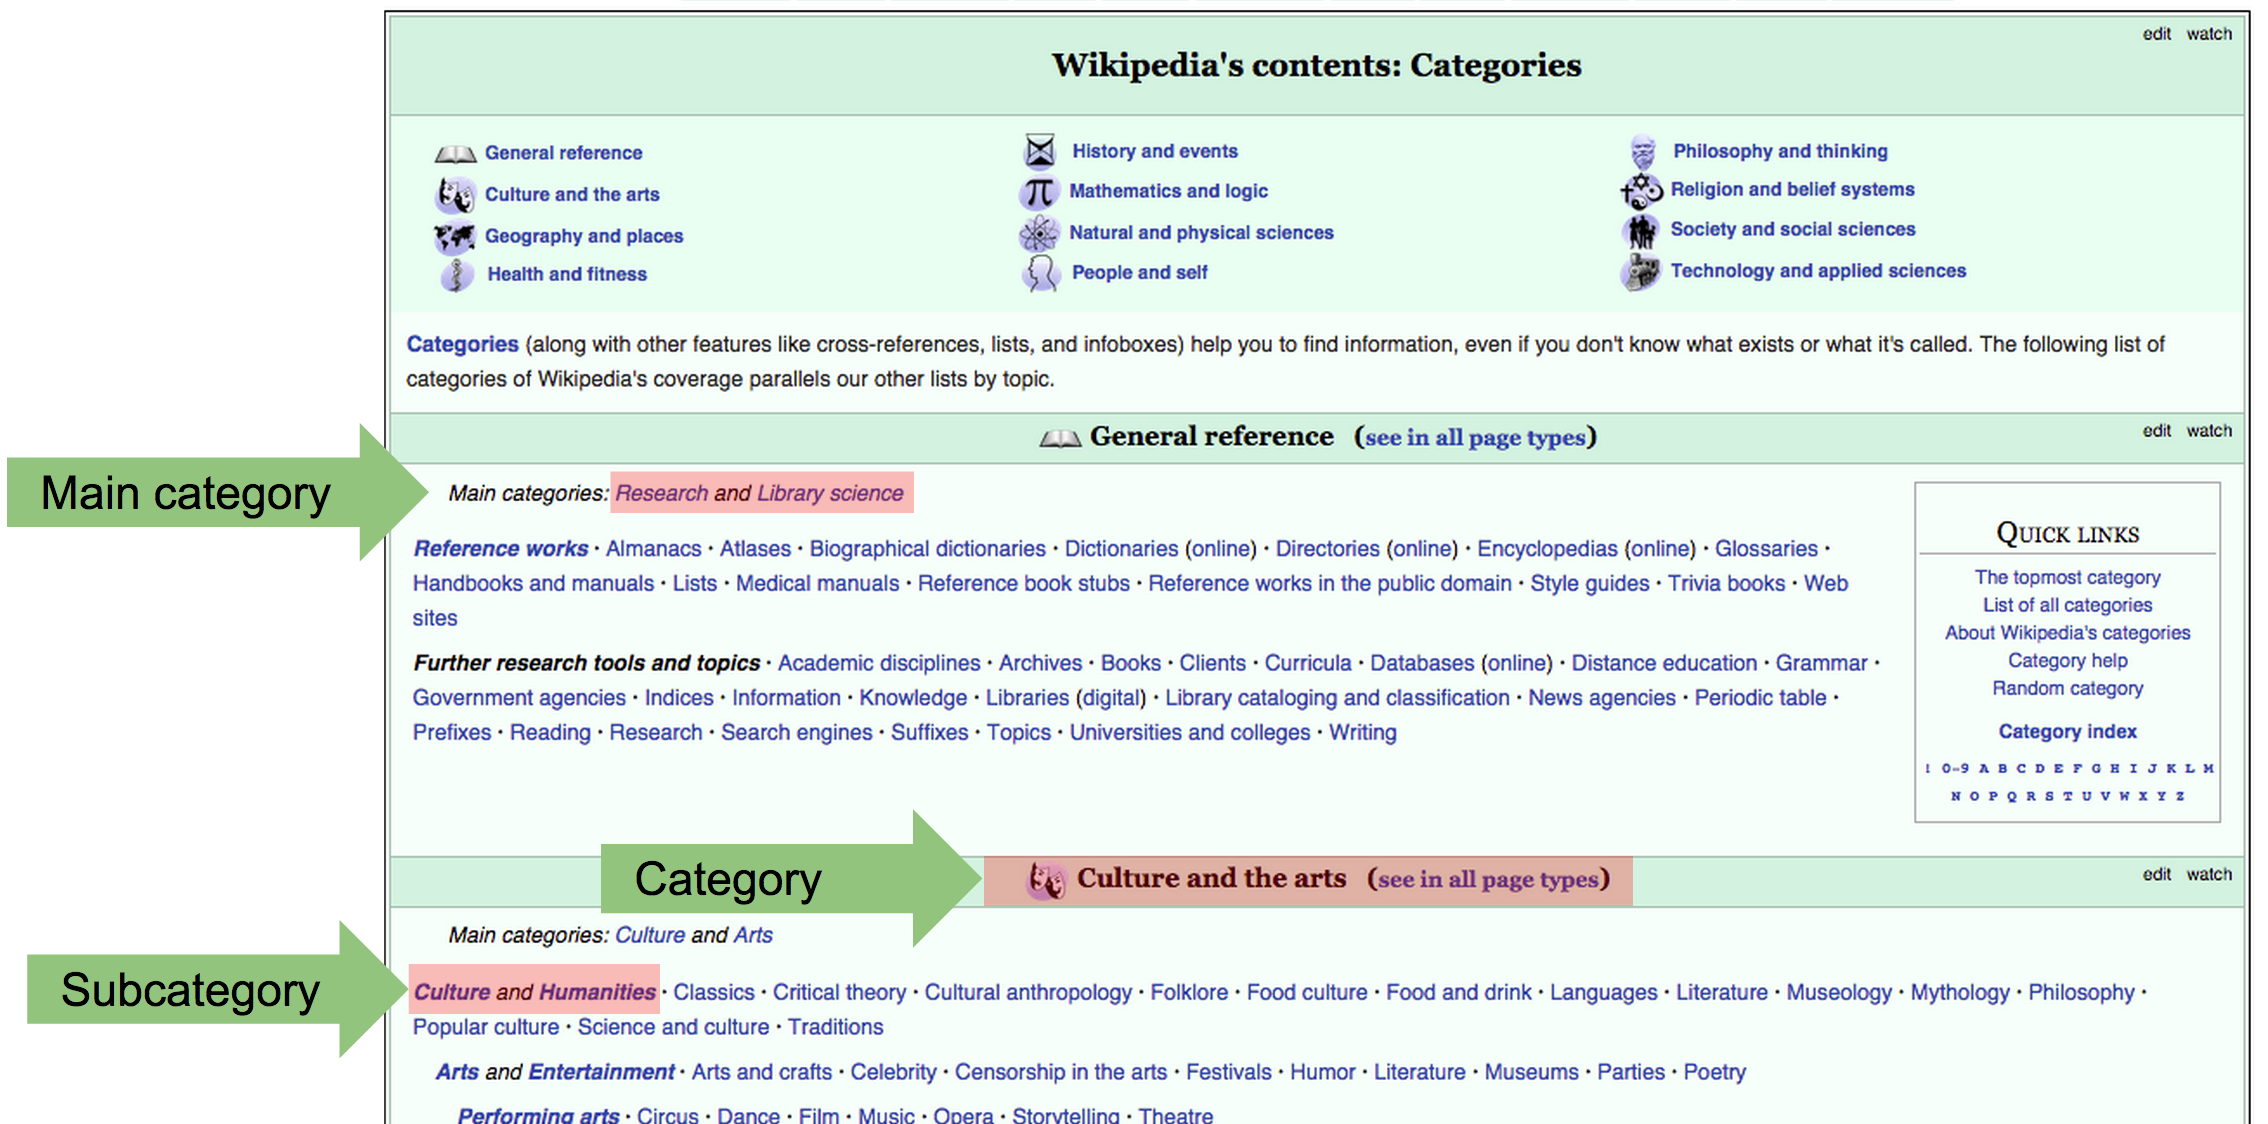
\includegraphics[width=1.0\textwidth]{1introduction/hierarchies-wikipedia-categories.png}
	\caption[Caption for LOF]{Wikipedia articles are structured in categories. For example, the article ``Bayes' theorem'' can be found in the hierarchy ``Bayesian statistics'' $<$ ``Statistics'' $<$ ``Mathematics and logic''.\footnotemark}
	\label{fig:1:hierarchies-categories}
\end{figure}

\footnotetext{Source: \url{https://en.wikipedia.org/wiki/Portal:Contents/Categories}}

\begin{figure}
	\centering
	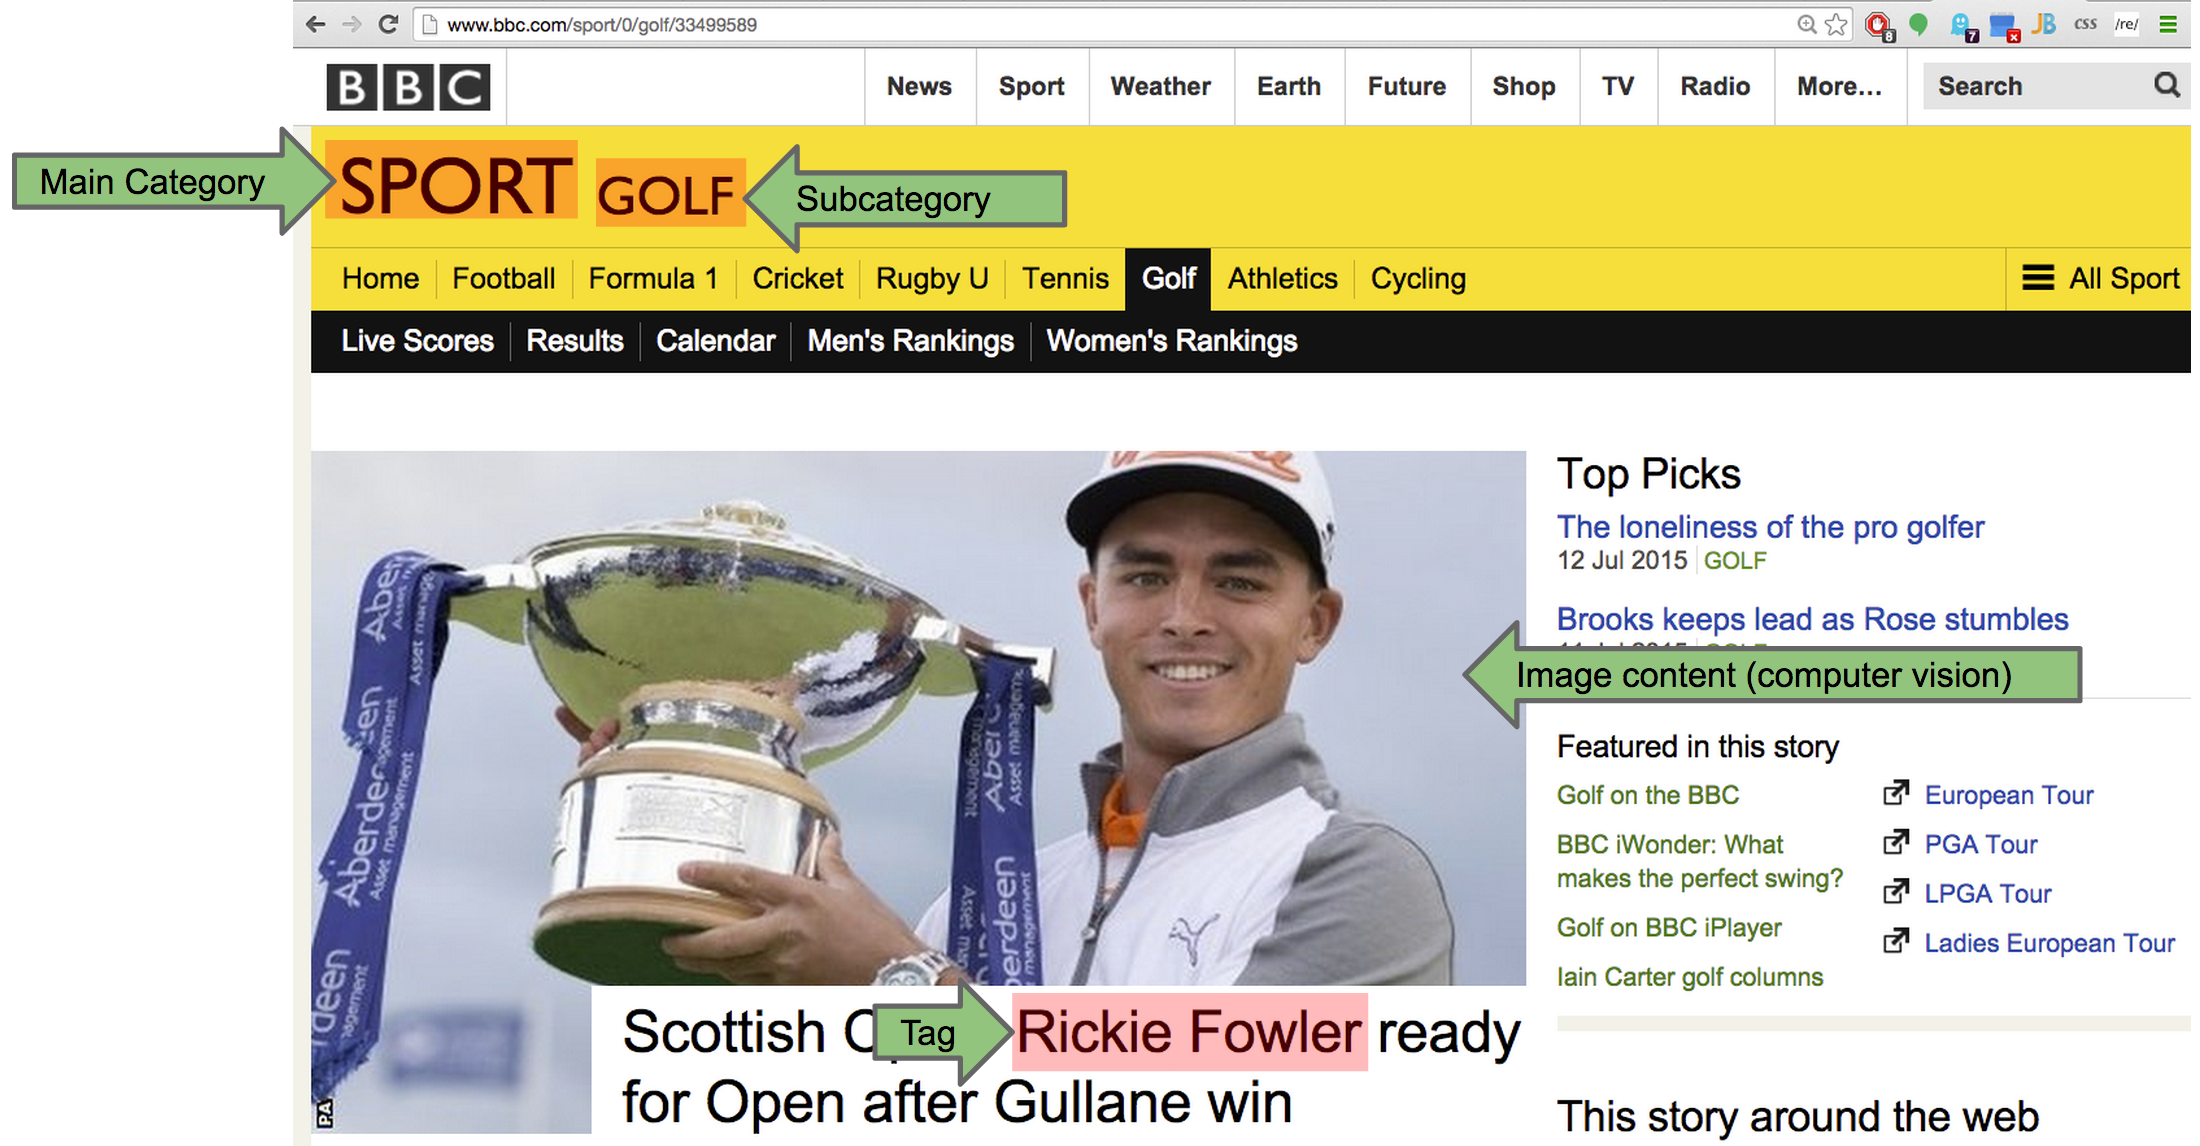
\includegraphics[width=1.0\textwidth]{1introduction/hierarchies-sports.png}
	\caption[Caption for LOF]{This sports article is categorized into the category ``sport'' and subcategory ``golf''. Additional tags (for example the name of the person who is on the picture) may also be available.\footnotemark}
	\label{fig:1:hierarchies-sports}
\end{figure}

This thesis is organized as follows: in Chapter~\ref{related-work}, related work underlying this thesis is discussed. Chapter~\ref{preliminaries} introduces theory needed to understand this thesis. Chapter~\ref{hierarchical-paragraph-vectors} investigates the formal core of this thesis by describing Hierarchical Paragraph Vectors. Chapter~\ref{experiments} describes the conducted experiments, and Chapter~\ref{conclusion-and-future-work} concludes the results and previews future work.

\newpage

\footnotetext{Source: \url{http://www.bbc.com/sport/0/golf/33499589}}

\chapter{Related Work}\label{related-work}

In this Chapter, the related research will be described. It will start with traditional and common representations, and describe their advantages and disadvantages. Next, more modern representations will be surveyed. Finally, publications describing hierarchical data will be described.

\section{Common Representations and Methods}

In NLP, probably the most widespread vector representation of text is the bag of words (BOW) representation~\cite{Harris1954}. For every word in the vocabulary, there is exactly one position in this vector, and if a word occurs $n$ times in a text, this component will be $n$ in the vector. Since the dimensionality of this vector is the size of the vocabulary, the BOW representation appeals by its simplicity. However, it suffers from high dimensionality, since the dimensionality is equal to the vocabulary size. Also sparsity is a major drawback, because a text block only contains a small fraction of all words in the vocabulary. Furthermore, the word order is lost, and therefore, different sentences with different meanings can have exactly the same representation.

Another commonly used representation is the bag-of-n-grams. While it mitigates some shortcomings of the BOW model, it also suffers from high dimensionality and sparsity.

Term frequency--inverse document frequency (TF--IDF) is a standard model in information retrieval. The term frequency is calculated by the number of times a word occurs in a document, while the inverse document frequency is the inverse of how often a word occurs in the whole corpus. The product of these two values is a weighted value, where rare words have a higher value when occurring in documents compared to frequently appearing words, for example stop words. Similar to the BOW model, a vector per document can be constructed by assigning a component of the vector per word in the corpus. Thus, it can be applied to any text. However, it also suffers from high dimensionality for the same reason as the BOW model does. To avoid this problem, the words can be ordered by term frequency, and only the top $n$ words are considered in the TF--IDF vector. Other words in this text are simply ignored. More information about TF--IDF can be found in~\ref{appendix:tf-idf} and in~\cite{Wu2008}.

For example, let us assume that we would like to produce word embeddings for the following documents.
\begin{displaymath}
\begin{array}{l|l}
\text{Document} & \text{Text} \\ 
\hline
d_1 & \text{The cat sleeps on the sofa.} \\
d_2 & \text{The mouse eats cheese.} \\
d_3 & \text{The cat tries to catch the mouse.} \\
\end{array}
\end{displaymath}
BOW produces the following word embeddings.
\begin{displaymath}
\begin{array}{l|rrrrrrrrrrr}
& \rotatebox[origin=l]{90}{the} &  \rotatebox[origin=l]{90}{cat} &  \rotatebox[origin=l]{90}{sleeps}  & \rotatebox[origin=l]{90}{on} &  \rotatebox[origin=l]{90}{sofa} & \rotatebox[origin=l]{90}{mouse} & \rotatebox[origin=l]{90}{eats} & \rotatebox[origin=l]{90}{cheese} & \rotatebox[origin=l]{90}{tries} & \rotatebox[origin=l]{90}{to} & \rotatebox[origin=l]{90}{catch} \\ 
\hline
d_1 & 2 & 1 & 1 & 1 & 1 & 0 & 0 & 0 & 0 & 0 & 0\\
d_2 & 1 & 0 & 0 & 0 & 0 & 1 & 1 & 1 & 0 & 0 & 0\\
d_3 & 2 & 1 & 0 & 0 & 0 & 1 & 0 & 0 & 1 & 1 & 1\\
\end{array}
\end{displaymath}
3-gram of words produces the following word embeddings.
\begin{displaymath}
\begin{array}{l|rrrrrrrrrrr}
& \rotatebox[origin=l]{90}{the cat sleeps} &  \rotatebox[origin=l]{90}{cat sleeps on} &  \rotatebox[origin=l]{90}{sleeps on the}  & \rotatebox[origin=l]{90}{on the sofa} &  \rotatebox[origin=l]{90}{the mouse eats} & \rotatebox[origin=l]{90}{mouse eats cheese} & \rotatebox[origin=l]{90}{the cat tries} & \rotatebox[origin=l]{90}{cat tries to} & \rotatebox[origin=l]{90}{tries to catch} & \rotatebox[origin=l]{90}{to catch the} & \rotatebox[origin=l]{90}{catch the mouse} \\ 
\hline
d_1 & 1 & 1 & 1 & 1 & 0 & 0 & 0 & 0 & 0 & 0 & 0\\
d_2 & 0 & 0 & 0 & 0 & 1 & 1 & 0 & 0 & 0 & 0 & 0\\
d_3 & 0 & 0 & 0 & 0 & 0 & 0 & 1 & 1 & 1 & 1 & 1\\
\end{array}
\end{displaymath}
TF-IDF produces the following word embeddings.
\begin{displaymath}
\begin{array}{l|rrrrrrrrrrr}
& \multicolumn{1}{c}{\rotatebox[origin=l]{90}{cat}} &  \multicolumn{1}{c}{\rotatebox[origin=l]{90}{catch}} &  \multicolumn{1}{c}{\rotatebox[origin=l]{90}{cheese}} & \multicolumn{1}{c}{\rotatebox[origin=l]{90}{eats}} & \multicolumn{1}{c}{\rotatebox[origin=l]{90}{mouse}} & \multicolumn{1}{c}{\rotatebox[origin=l]{90}{on}} & \multicolumn{1}{c}{\rotatebox[origin=l]{90}{sleeps}} & \multicolumn{1}{c}{\rotatebox[origin=l]{90}{sofa}} & \multicolumn{1}{c}{\rotatebox[origin=l]{90}{the}} & \multicolumn{1}{c}{\rotatebox[origin=l]{90}{to}} & \multicolumn{1}{c}{\rotatebox[origin=l]{90}{tries}} \\ 
\hline
d_1 & 0.34 & 0.0 & 0.0 & 0.0 & 0.0 & 0.45 & 0.45 & 0.45 & 0.53 & 0.0 & 0.0\\
d_2 & 0.0 & 0.0 & 0.58 & 0.58 & 0.44 & 0.0 & 0.0 & 0.0 & 0.35 & 0.0 & 0.0\\
d_3 & 0.32 & 0.42 & 0.0 & 0.0 & 0.32 & 0.0 & 0.0 & 0.0 & 0.5 & 0.42 & 0.42\\
\end{array}
\end{displaymath}

Finally, all the representations discussed above (BOW, bag-of-n-grams, TF--IDF) do not capture the semantics of words. For example, the words ``fast'' and ``quick'' are as far apart from each other as they are from the word ``blue'', even though the words ``fast'' and ``quick'' are semantically more similar to each other. It is even more surprising that such na{\"\i}ve models can perform relatively well.

\section{Neural Networks for Language Models}

The theory underlying artificial neural networks has been existing for a long time~\cite{Ackley1985, LeCun1985, Rumelhart1986}. The two fundamental concepts for these networks are gradient descent and backpropagation. Feedforward neural network language models (NNLM) build on this technique and have deeply studied and tuned in recent publications~\cite{Bengio2006, Collobert2008, Mnih2009, Turian2010}. These NNLMs have been shown to outperform the n-gram models significantly. One major drawback of these techniques is that they are computationally expensive, and thus slow to train and test.

In 2013, Mikolov et al.\ published~\cite{Mikolov2013a}, where they describe the recurrent neural network language model (RNNLM). This network helps to overcome some shortcomings of the NNLM\@. Specifically, it has a short-term memory, and thus can model more complex behavior than shallow neural networks~\cite{Kombrink2011}~\cite{Bengio2007}. A disadvantage of RNNs is their greater need for resources and thus prohibitively large computational cost. However, Mikolov et al.\ managed, with the help of approximate algorithms and an optimized implementation, to massively reduce computational complexity. The result of this are two new models, summarized under the name Word2vec: continuous bag-of-words models (CBOW) and continuous skip-gram models (skip-gram). More information about these models can be found in Chapter~\ref{preliminaries}.

In their paper~\cite{Le2014} in 2014, Le and Mikolov extended the CBOW and Skip-gram model by a paragraph vector. This new vector enables arbitrary blocks of text (for example articles, paragraphs, sentences) to learn and share a common vector, which acts as a memory to learn the word vectors. The CBOW model that is extended by the paragraph vector (PV) is called PV-DBOW, while the extended Skip-gram model is called Distributed Memory Model of Paragraph Vectors (PV-DM). The name ``distributed memory'' originates from the fact that the paragraph vector acts as a memory for the current context. These two models are also known as Doc2vec.

\section{Alternative Word Embedding Models}

In~\cite{Goldberg2014a}, the authors analyze the skip-gram model with negative sampling. They suggest that the embedding method by Mikolov et al.\ is implicitly factorizing a word-content matrix, and they attempt to implement this factorization directly. They conclude that their factorization method is better suited to optimize the objective by Mikolov et al. However, their model does not perform well on the word anology task.

In~\cite{Pennington2014}, the authors present the Global Vectors model (GloVe). Their model is a combination of matrix factorization methods and local context window methods. Though their model works differently compared to the model by Mikolov et al., the two models perform similarly well. In~\cite{Shi2014}, the authors link the model by Mikolov et al.\ with GloVe by explaining out the similarities and the differences.

\section{Exploiting Hierarchies}

There have been many approaches to using hierarchies for NLP, specifically with NNLMs. However, to the best knowledge of the author, hierarchies have not yet been combined with the paragraph vectors of~\cite{Le2014}.

In~\cite{Luong2013}, the authors build a hierarchy of single words by modeling the morphemic compositionality, which can be seen as a specialization of HPV\@.

In~\cite{Morin2005}, the authors use clustered words from WordNet~\cite{Fellbaum1998} by hierarchically decomposing the conditional probabilities as an alternative for importance sampling to speed up the training of the word embeddings. Furthermore,~\cite{Mnih2009} extended the ideas in~\cite{Morin2005}.

%todo tbd carsten: recheck
In~\cite{Fu2014}, the authors use word embeddings, obtained by skip-gram, to learn semantic hierarchies. They claim that hierarchical information is encoded in word embeddings. This encourages the use of existing hierarchies to improve the quality of word embeddings.

%todo low prio: go more in depth. q: cite more? a: not neccessarily more, buy you may ment to go deeper for the relevant existing citations on word embeddings.


% cite more in depth?
%\section{Cite more?}
%[Linguistic Regularities in Continuous Space Word Representations]?
%[Hierarchical Reasoning with Distributed Vector Representations]
%[Hierarchical Neural Language Models for Joint Representation of Streaming Documents and their Content]
%[Deep Recursive Neural Networks for Compositionality in Language]
%\href{http://arxiv.org/pdf/1504.05070v2.pdf}{\emph{http://arxiv.org/pdf/1504.05070v2.pdf}}
%\href{http://www.aclweb.org/website/old_anthology/W/W96/W96-0103.pdf}{\emph{http://www.aclweb.org/website/old\_anthology/W/W96/W96-0103.pdf}}
%\href{http://dl.acm.org/citation.cfm?id=993390}{\emph{http://dl.acm.org/citation.cfm?id=993390}}

\chapter{Preliminaries}\label{preliminaries}

In this Chapter, the models, algorithms and objectives of the two basic word embedding algorithms Word2vec and Doc2vec are described.

\section{Word2vec}

The term Word2vec summarizes two different models: the distributed bag of words model (CBOW) and the continuous skip-gram model (skip-gram). Both use neural networks, and they work very similarly. However, they have very different objectives and thus are able to capture different syntactic and semantic patterns. Furthermore, they both have different parameters. Let us have a closer look.

\subsection{Objectives}

In the paper, two different objectives for the CBOW model are proposed. Mathematically, this can be expressed in two formulas, where $w_{j}$ is the $j$-th word, and $c$ is the window size. The first objective is to predict the next word-based on $c$ previously encountered words.
\begin{displaymath}
  \underset{W}{\text{maximize}}\ p(w_{t} | w_{t - c},\ w_{t - (c-1)},\ \ldots,\ w_{t - 2},\ w_{t - 1})
\end{displaymath}
The second objective is to predict the word in the middle of $c$ previously encountered words and $c$ following words.
\begin{displaymath}
  \underset{W}{\text{maximize}}\ p(w_{t} | w_{t - c},\ w_{t - (c-1)},\ \ldots,\ w_{t - 1},\ w_{t + 1},\ \ldots,\ w_{t + (c-1)},\ w_{t + c})
\end{displaymath}
In this thesis, CBOW will always use the second objective, which is predicting the middle word from surrounding words. This leads to the objective of maximizing the average log probability.
\begin{displaymath}
 \underset{W}{\text{maximize}}\ \frac{1}{T} \sum_{t=1}^{T}\ \sum_{-c \leq j \leq c, j \neg 0} \log p(w_{t}|w_{t + j})
\end{displaymath}

While the CBOW model tries to predict the middle word given a context, the skip-gram model tries to do the opposite, which is to predict the surrounding words given a single word.
\begin{displaymath}
  \underset{W}{\text{maximize}}\ p(w_{t - c},\ w_{t - (c-1)},\ \ldots,\ w_{t - 1},\ w_{t + 1},\ \ldots,\ w_{t + (c-1)},\ w_{t + c} | w_{t})
\end{displaymath}
Again, this leads to the objective of maximizing the average log probability.
\begin{displaymath}
 \underset{W}{\text{maximize}}\ \frac{1}{T} \sum_{t=1}^{T}\ \sum_{-c \leq j \leq c, j \neg 0} \log p(w_{t + j}|w_{t})
\end{displaymath}

\subsection{Neural Network Language Model}

To achieve the objectives described above, one recurrent neural network per objective is used. In the next few paragraphs, the neural network for the CBOW model is described. The neural network for the skip-gram model works analogous. The differences to the CBOW model are described at the end of this subsection.

The neural network consists of four layers: one input layer $I$, one projection layer $P$, one hidden layer $H$, and one output layer $V$. To model the weights of the connections between each connected layer, we use matrices. Since each two connected layers are fully connected to each other, the dimensionality of these matrices is the dimensionality of the upper layer times the dimensionality of the lower layer.

\begin{figure}
	\centering
	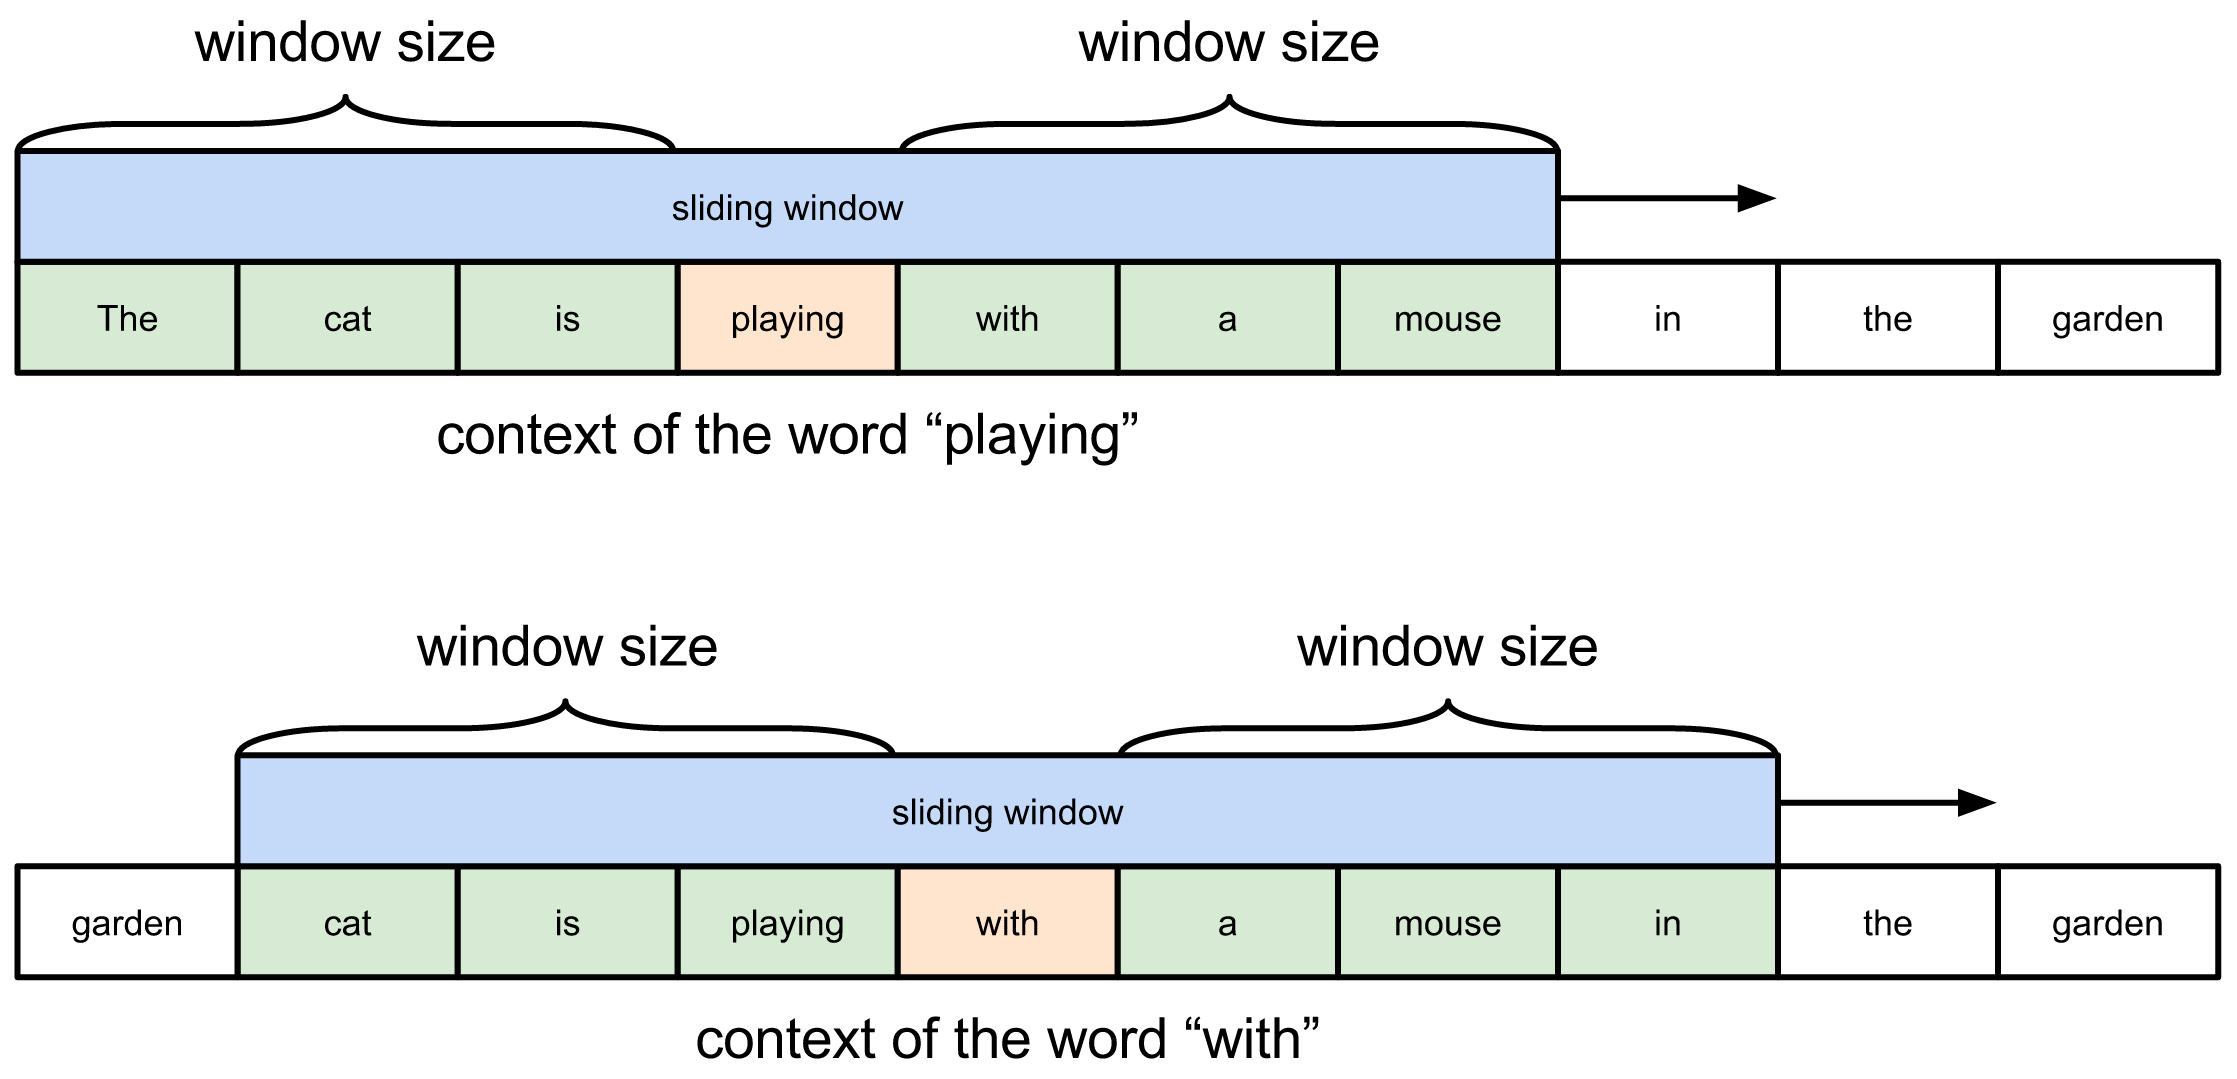
\includegraphics[width=0.9\textwidth]{3preliminaries/sliding-window}
	\caption{The window size of the sliding window defines which words are in the context of the middle word.}
	\label{fig:3:sliding-window}
\end{figure}

In the input layer, all words in the context of a word are listed, while the context is defined by the window size $c$. For example, if $c=3$, then the context for the word ``playing'' of the sentence ``The cat is \emph{playing} with a mouse in the garden'' is [the, cat, is, with, a, mouse], and the context for the word ``with'' is [cat, is, playing, a, mouse, in], see Figure~\ref{fig:3:sliding-window}. Therefore, the dimensionality of $I$ is two times the window size $c$.
\begin{displaymath}
\dim(I) = 2c
\end{displaymath}

Next, every word in the context is mapped to a $d$ dimensional vector, where $d$ is the word vector dimensionality. The weights of this projection define the resulting word vector. The dimensionality of the projection layer is the dimensionality of the input layer times the word vector dimensionality.
\begin{displaymath}
\dim(P) = \dim(I) \times d = 2c \times d
\end{displaymath}

An equivalent model of the input and projection layer is to use the whole vocabulary $U$ as input layer, while the words in the context are encoded with a 1 and the ones not in the context with a 0. Then the projection layer consists of all word vectors, and thus does not have to be changed when the context words change. Since the words that are not in the context are encoded as 0, the corresponding word vectors are multiplied by 0 and thus do not contribute to the prediction.

The hidden layer is fully connected to the projection layer, and has arbitrary dimensionality, usually between 500 and 2000.
\begin{displaymath}
\dim(H) = x \in [500,\ 2000]
\end{displaymath}

Finally, the output layer has the same dimensionality as $U$, where the $j$-th value $v_{j}$ is a score to calculate the conditional probability that the $j$-th word $w_{j}$ occurs given the context $w_{x - c},\ \ldots\ ,w_{x + c}$. In the next subsection, we describe how to calculate these conditional probabilities.
\begin{displaymath}
\dim(V) = \dim(U)
\end{displaymath}

Now let us consider the skip-gram model. The input layer consists of only one word, and the projection and the hidden layer have the same architecture and meaning as in the CBOW model. However, instead of having only one multinomial distribution, we have $2c$ multinomial distributions, one for each word in the context. Thus, the dimensionality of the neural network for CBOW is different.
\begin{displaymath}
\begin{aligned}
\dim(I) &= 1 \\
\dim(P) &= d \\
\dim(H) &= x \in [500,\ 2000] \\
\dim(V) &= 2c \times \dim(U)
\end{aligned}
\end{displaymath}

\subsection{Algorithm}

As in the common neural network, the weights are learned via gradient descent and backpropagation. Let us again consider the algorithm for the CBOW\@. First, each word vector (one per word) is initialized randomly. Next, the documents are processed using a sliding window of size $c$ (usually between 5 and 20). Then, the word vectors of the context are set as the projection layer, and the network tries to predict the middle word. The error gradient is then calculated and backpropagated by using soft-max. $v_j$ is the value in the output layer per word in the vocabulary $U$.
\begin{displaymath}
p(w_{t} | w_{t - c},\ \ldots,\ w_{t + c}) = \frac{e^{v_{j}}}{\sum_{j'=1}^{\dim(U)}\ e^{v_{j'}}}
\end{displaymath}

This conditional probability is then compared to the actual output (the middle word). Based on the result (overestimation or underestimation), the error is backpropagated through the neural network, and the weights for the word vectors in this context are updated accordingly.

For example, consider again the sentence ``The cat is playing with a \emph{mouse} in the garden'' with a window size $c=3$ and the word to predict being ``mouse''. If the network predicts that the word ``cat'' is probable to appear (however, ``cat'' does not appear in the context of ``mouse''), then this error is backpropagated and the word vectors for [playing, with, a, in, the, garden] are updated. In contrast, if the word ``mouse'' is predicted to be appearing in this context, the error is small and thus the backpropagation will not change the vectors [playing, with, a, in, the, garden] significantly.

The skip-gram algorithm works analogously to the CBOW model. It tries to predict the context of $w_{j}$, and backpropagates the mean error to change the word vector of $w_{j}$ accordingly.

\begin{figure}
	\centering
	\begin{subfigure}{.5\textwidth}
		\centering
		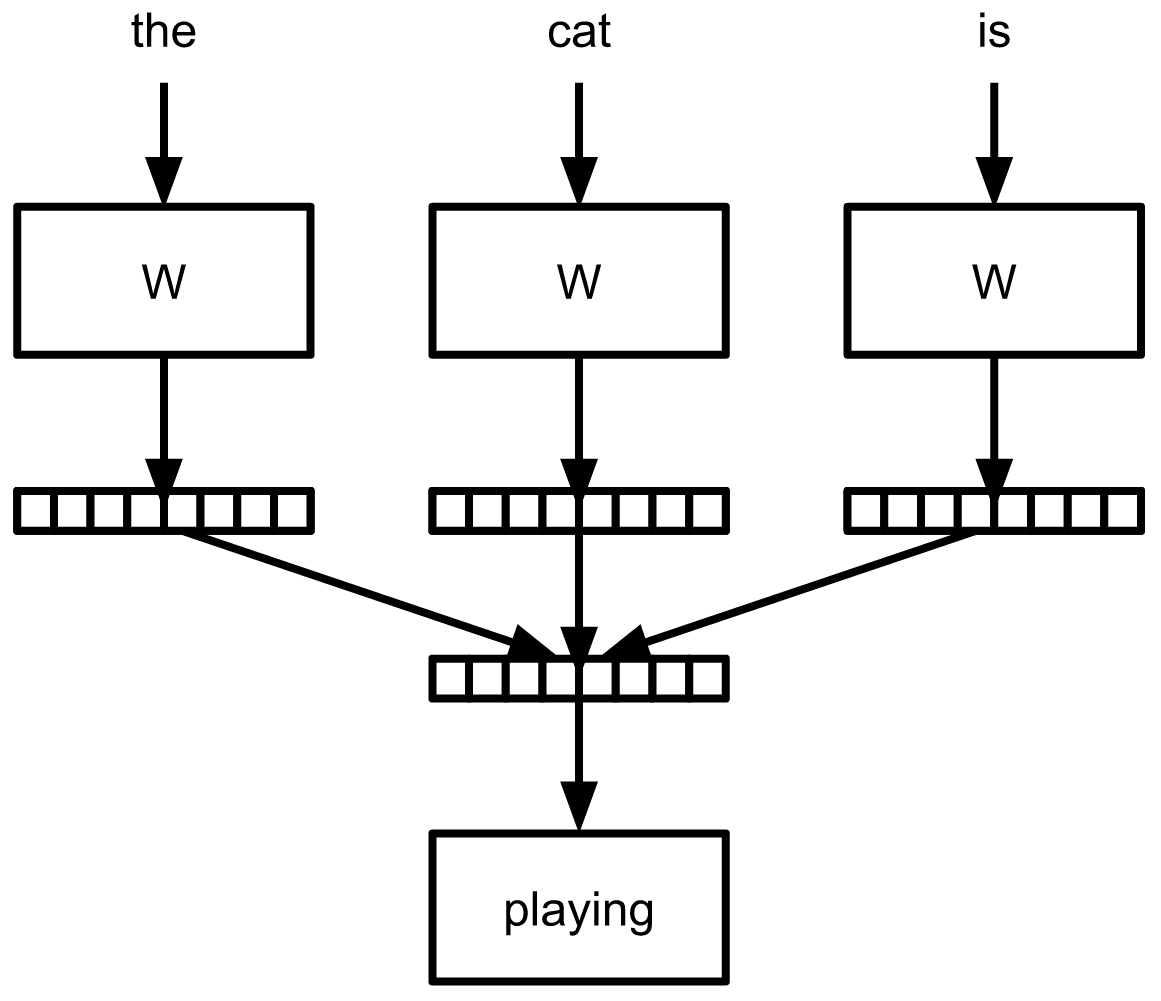
\includegraphics[width=1.0\linewidth]{3preliminaries/cbow}
		\caption{CBOW}
		\label{fig:3:cbow}
	\end{subfigure}\begin{subfigure}{.5\textwidth}
		\centering
		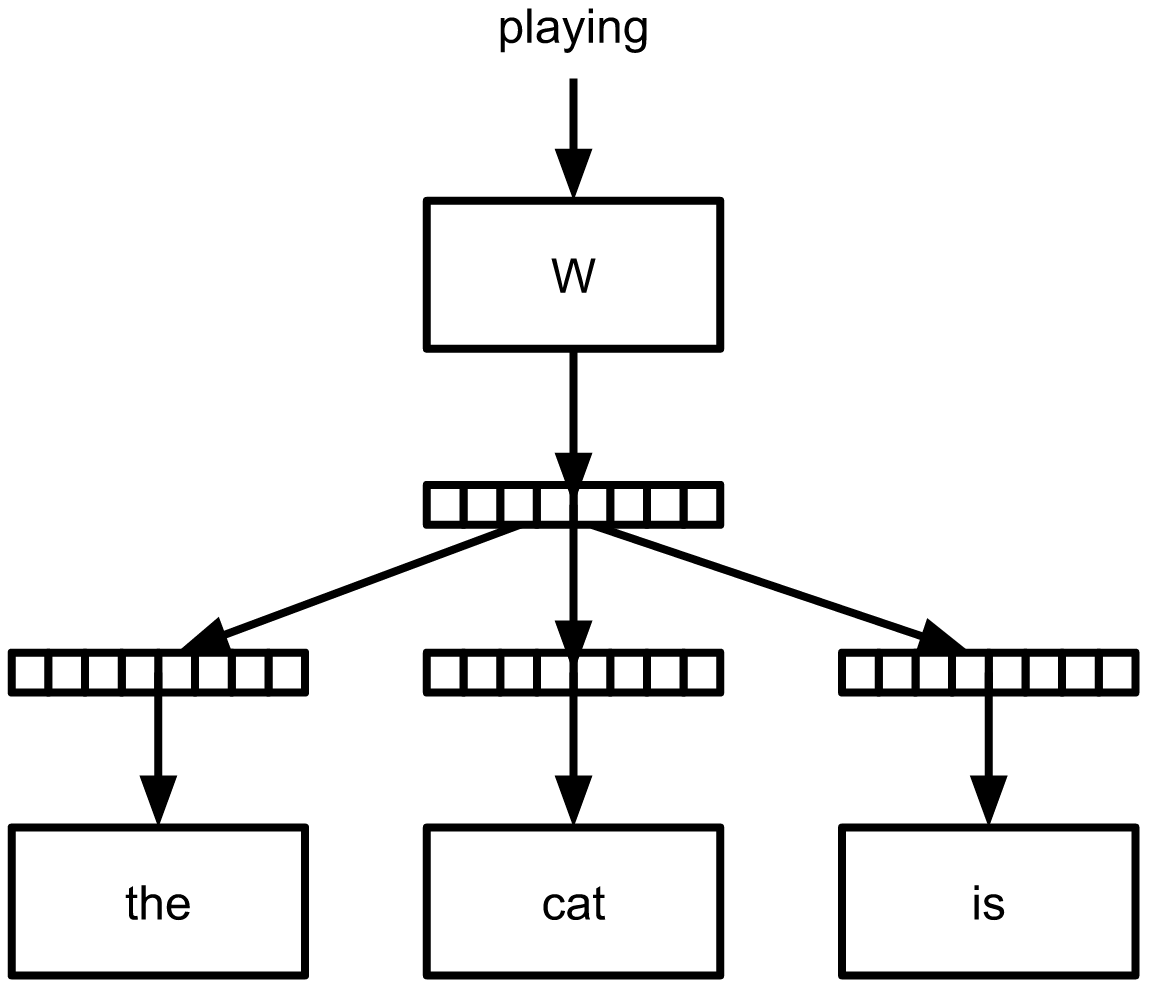
\includegraphics[width=1.0\linewidth]{3preliminaries/sg}
		\caption{Skip-gram}
		\label{fig:3:sg}
	\end{subfigure}
	\caption{The architecture of the neural network for CBOW and skip-gram. On the top is the input layer, in the middle the hidden layer, and in the bottom the output layer.}
	\label{fig:3:cbow-sg}
\end{figure}

The two architectures are sketched in Figure~\ref{fig:3:cbow-sg}. For a more extensive description on how exactly the Word2vec parameters are learned, see~\cite{Mikolov2013a, Mikolov2013, TomasMikolov, Rong2014, Goldberg2014a}.

\subsection{Computational Optimizations}

%resolved repetition:  Furthermore, the ultimate generalization is to train on an infinite amount of data, and thus being able to process a vast amount of text in a short time is a huge advantage.
While the two models CBOW and skip-gram discussed above are useful for understanding the basic models, these algorithms are computationally very inefficient. This is especially true when the vocabulary is large. Since there are nearly infinite amounts of written text available (for example Wikipedia, books, news, blogs) to train word embeddings on, it is imperative to minimize computational complexity in order to maximize accuracy by processing more text in less time. In this subsection, we will briefly describe the theoretical optimizations. As we will later see in Chapter~\ref{experiments}, additional optimizations regarding the implementation are also key to good results.

Since these optimizations are not necessary for understanding this thesis, we will only very briefly describe each concept. Interested readers can refer to~\cite{Mikolov2013, Rong2014, Goldberg2014a} to understand these optimizations in greater depth.

\emph{Hierarchical soft-max}~\cite{Morin2005, Mnih2009} calculates an approximated soft-max more efficiently.

\emph{Negative sampling}~\cite{Mikolov2013, Goldberg2014a} is a replacement for the soft-max and samples for every word $w_{j}$ $n$ words (usually between 5 and 20) from the vocabulary which are assumed not to appear with $w_{j}$.

Finally, \emph{sub-sampling of frequent words}~\cite{Mikolov2013} favors rare words compared to frequent words, as rare words are more probable to contribute important information compared to frequent words like stop words. This is similar to the IDF part of TF-IDF\@.

\section{Doc2vec}

As described in the previous section, Word2vec works with a sliding window of a fixed size. Again, let us consider the sentence ``The cat is playing with a mouse in the garden.''. If $c=3$, the words ``cat'' and ``garden'' will never occur together, and thus their respective word vectors will not be close to each other.

Doc2vec changes exactly that by adding an additional paragraph vector to each ``paragraph''. But let us first describe what is meant by a paragraph: a ``paragraph'' is a text block with arbitrary length, for example a chapter, a section, a text paragraph or a sentence. In this section, the word ``paragraph'' should describe such a text block of arbitrary length, and a paragraph vector (PV) is a vector for such a paragraph, like a word vector is to a word.

Let us continue with the paragraph vector characterization. This paragraph vector serves as a common context, which is shared within the paragraph. In the previous example ``The cat is playing with a mouse in the garden.'', the paragraph vector allows to share a context between ``cat'' and ``garden''. This vector can also be thought of as a word which appears in the context of a larger entity than the sliding window size allows.

One key advantage of Doc2vec is that it can easily be built into Word2vec. Essentially, each paragraph vector is a word vector which appears in every context of the current paragraph. It can be trained the same way as the word vectors through gradient descent and backpropagation, using the same neural network.

The PV enhanced CBOW model is called paragraph vector distributed memory (PV-DM) to stress the role of the PV to act as distributed memory. For the skip-gram model, the PV enhanced model is called PV-DBOW and is illustrated in Figure~\ref{fig:3:pv-dbow-pv-dm}.

\begin{figure}
	\centering
	\begin{subfigure}{.575\textwidth}
		\centering
		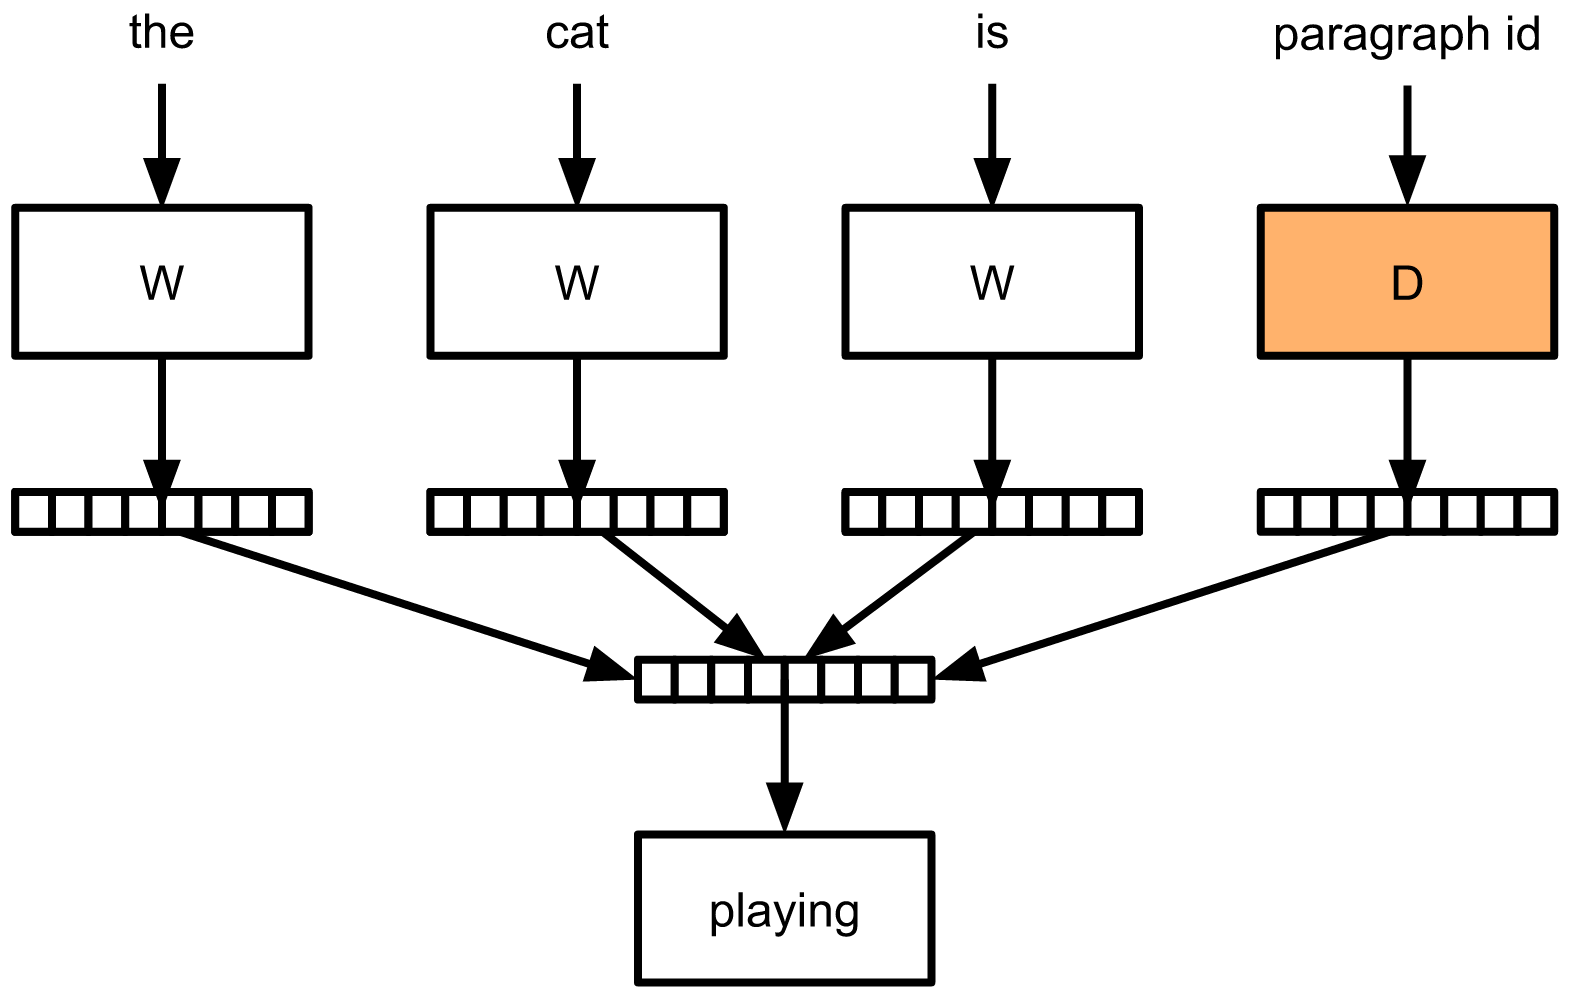
\includegraphics[width=1.0\linewidth]{3preliminaries/pv-dm}
		\caption{PV-DM}
		\label{fig:3:pv-dm}
	\end{subfigure}\begin{subfigure}{.425\textwidth}
	\centering
	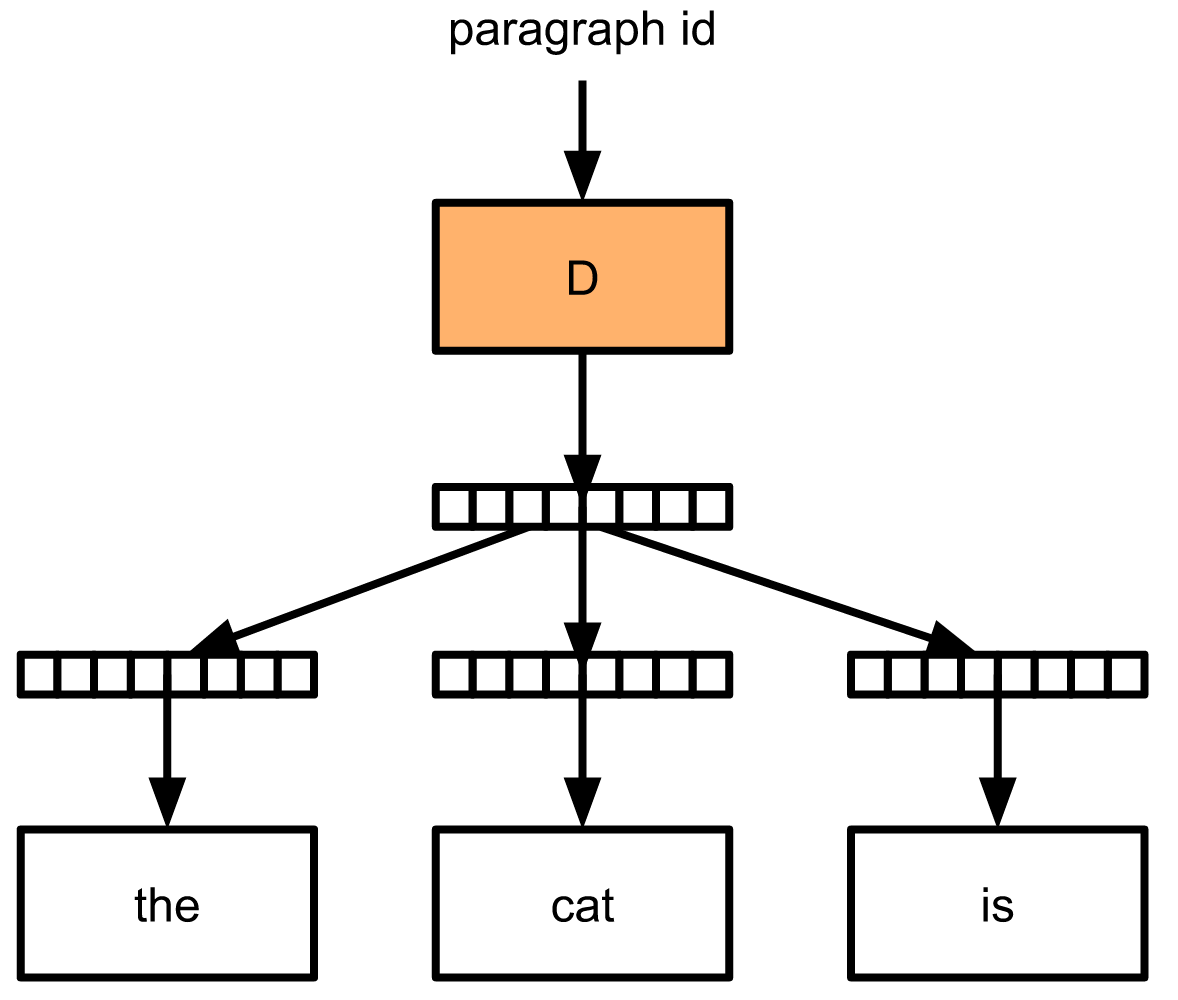
\includegraphics[width=1.0\linewidth]{3preliminaries/pv-dbow}
	\caption{PV-DBOW}
	\label{fig:3:pv-dbow}
	\end{subfigure}
\caption{The architecture of the neural network for PV-DM and PV-DBOW\@. On top is the input layer, in the middle the hidden layer, and in the bottom the output layer.}
\label{fig:3:pv-dbow-pv-dm}
\end{figure}

\chapter{Hierarchical Paragraph Vectors}\label{hierarchical-paragraph-vectors}

\section{Hierarchies and NLP}\label{hierarchies-and-nlp}

Today, there is a vast amount of text available to be used in NLP\@. Many texts (for example articles, websites, books, comments, reviews and messages), are naturally divided into sub-texts (for example chapters, sections, paragraphs and sentences). Furthermore, they are usually also categorized or tagged (for example by authors, publishers, domain names, references, topics and genres).

Consider for example a book about how to learn programming Ruby. This book is divided into multiple chapters, which, in turn, are divided into multiple sections and sentences. Furthermore, this book is found on Amazon in the category ``Programming'', which, in turn, can be found in ``Computers \& Technology'', as can be observed in Figure~\ref{fig:4:book-example}.

Now what do these hierarchies represent? The structure represents concepts and abstractions, which represent potentially useful information. For example, if a person reads multiple articles about the French revolution, they can better predict which words will appear the next article about the French revolution. Thus, if this information can be used to learn the word embeddings, it lends itself for exploitation in the training of word embeddings.

\begin{figure}
	\centering
	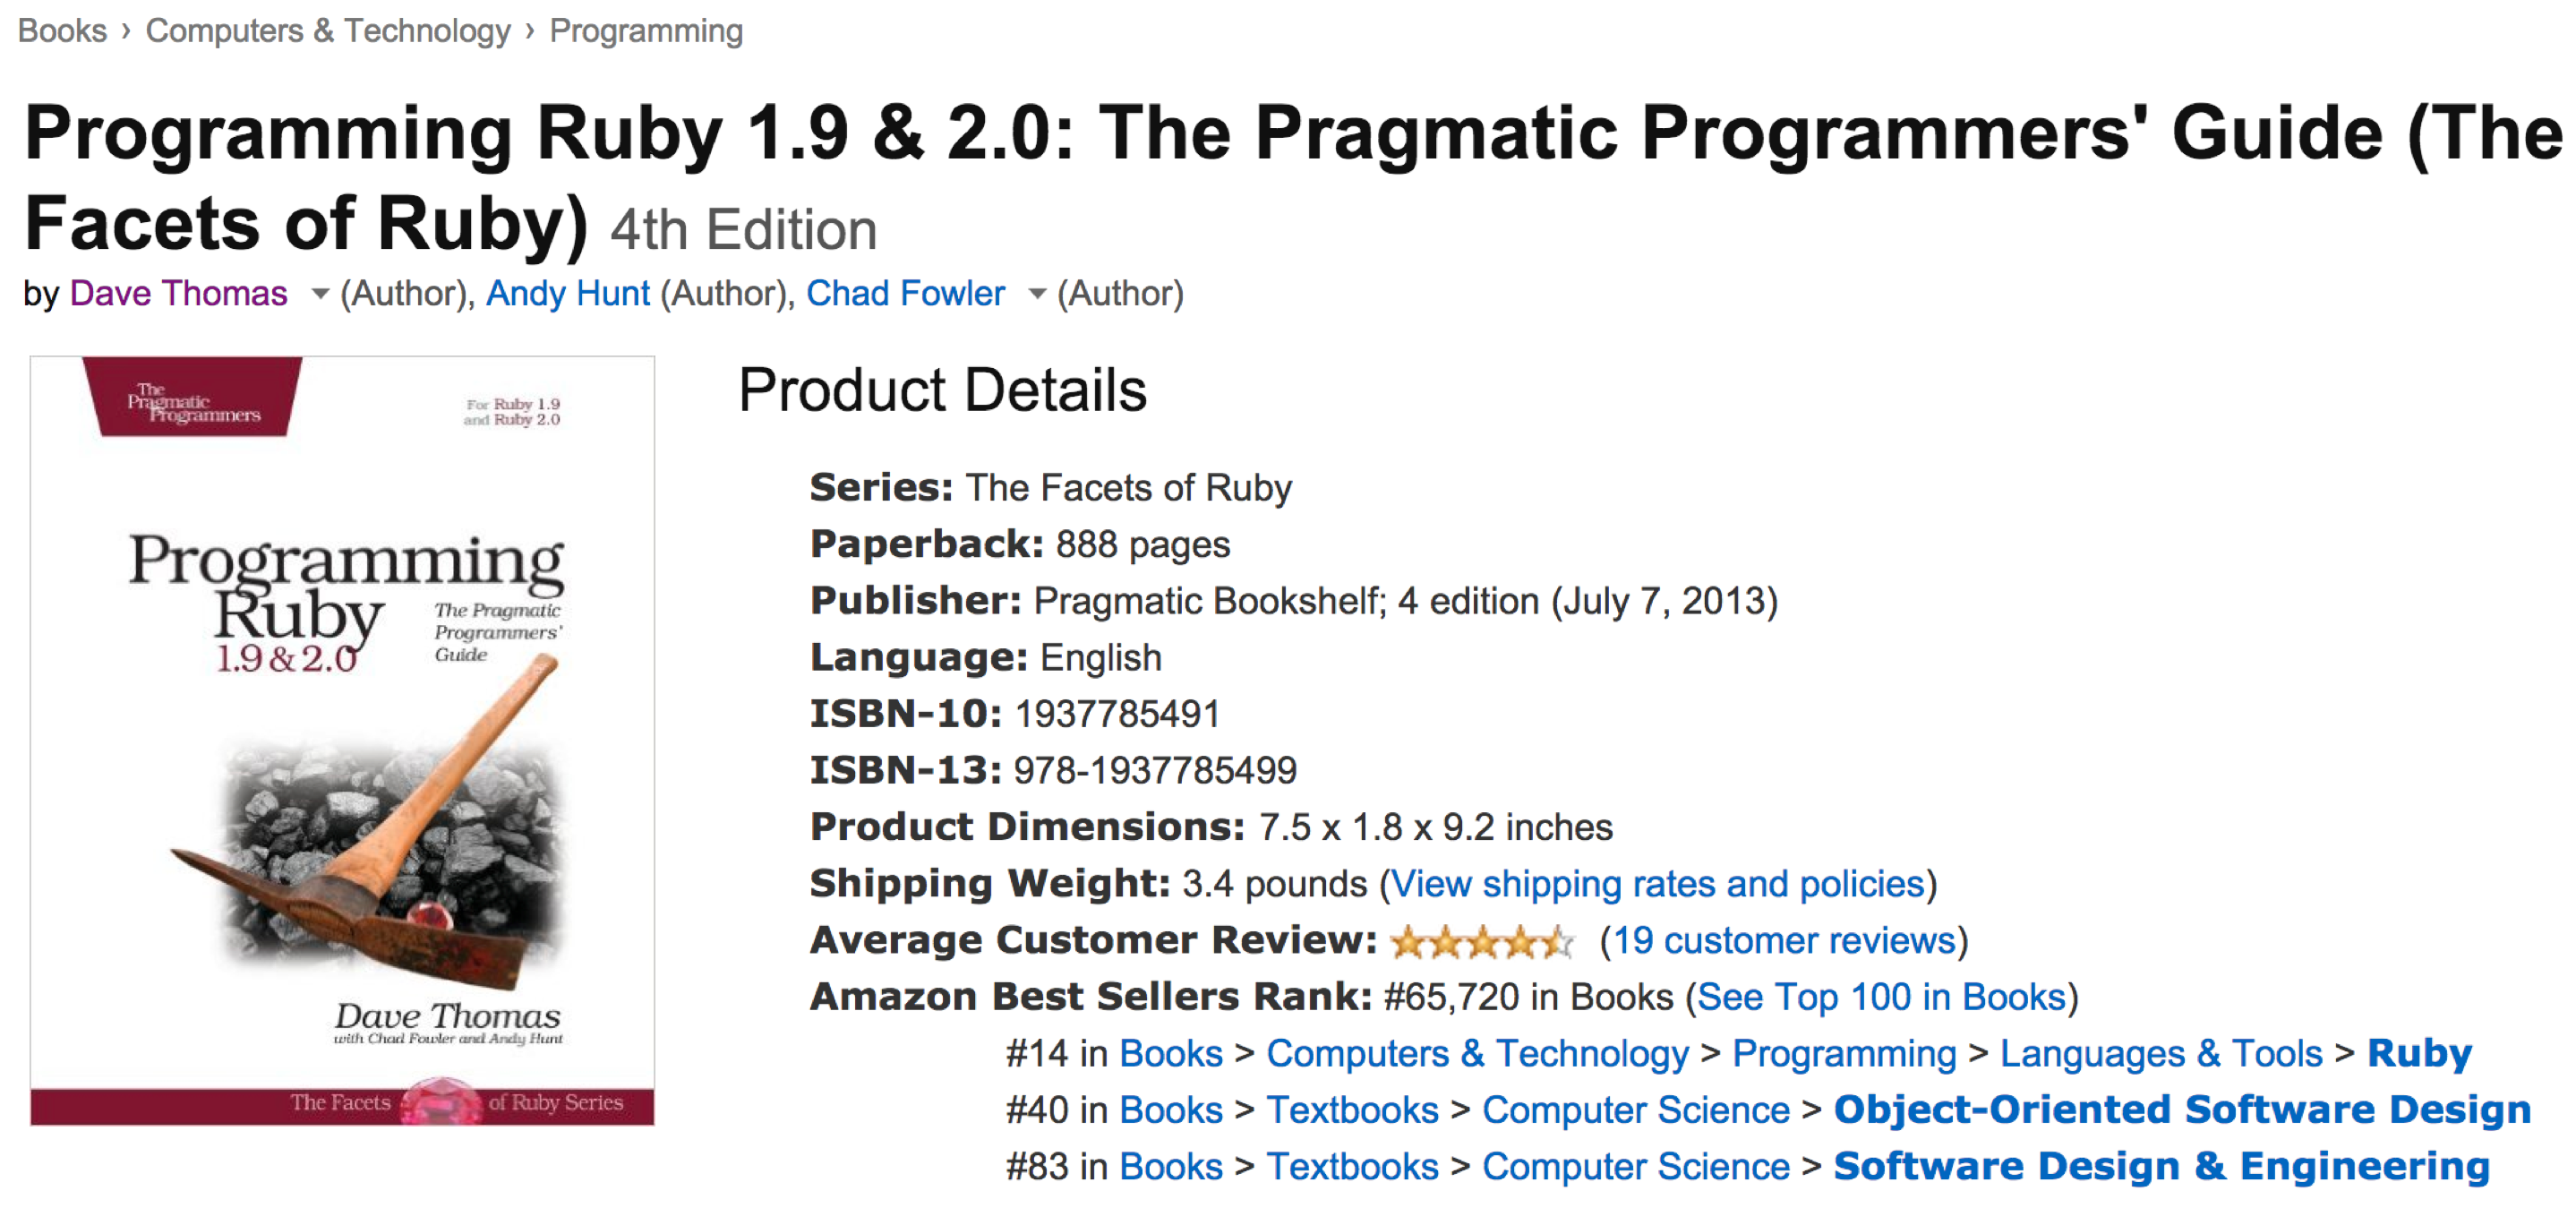
\includegraphics[width=0.9\textwidth]{4hpvs/book-example.png}
	\caption[Caption for LOF]{This book is categorized into ``Programming'' (on the very top of the image), ``Ruby'', ``Object-Oriented Software Design'' and ``Software Design \& Engineering'', which, in turn, can be found in their respective parent category. There are also additional attributes, for example the language of the book and the authors.\footnotemark}
	\label{fig:4:book-example}
\end{figure}

\section{Obtaining Hierarchies}\label{obtaining-hierarchies}

From the perspective of a document, there are potentially two directions in which hierarchies are found. One is ``upwards'', and the other is ``downwards''. Let us define what we mean by that, and how these hierarchies can be obtained.

``Upwards'' refers to hierarchies across multiple documents. As stated above, natural hierarchies are for example author names, publishers, domain names, references, topics or genres. Where available, these can be obtained directly from the data. If this data is not available, it could be generated artificially by standard machine learning methods, for example by Latent Dirichlet Allocation (LDA).

``Downwards'' describes hierarchies to be found within a single document. These could for example be chapters, paragraphs or sentences. These hierarchies are also often available directly through the data, or can be obtained by parsing the text or markup. For example, when an HTML document is given, the HTML tags (for example h1, h2, h3, p, br) can be used to split the text into multiple blocks, and the resulting text blocks can be parsed and split up by sentence.

\footnotetext{Source: \url{http://www.amazon.com/gp/product/1937785491}}

\section{Algorithms}\label{algorithms}

\subsection{HPV-DM}\label{hpv-dm}

HPV-DM builds upon PV-DM\@. Instead of only allowing one paragraph vector per context, it allows multiple hierarchical paragraph vectors for the same context, as can be seen in Figure~\ref{fig:4:hpv-dm}. Additionally, some hierarchical paragraph vectors appear multiple times in different contexts. Similar to the paragraph vectors, the hierarchical paragraph vectors can be thought of as additional memory for the current context, or as additional words which are always present in some context.

\begin{figure}
	\centering
	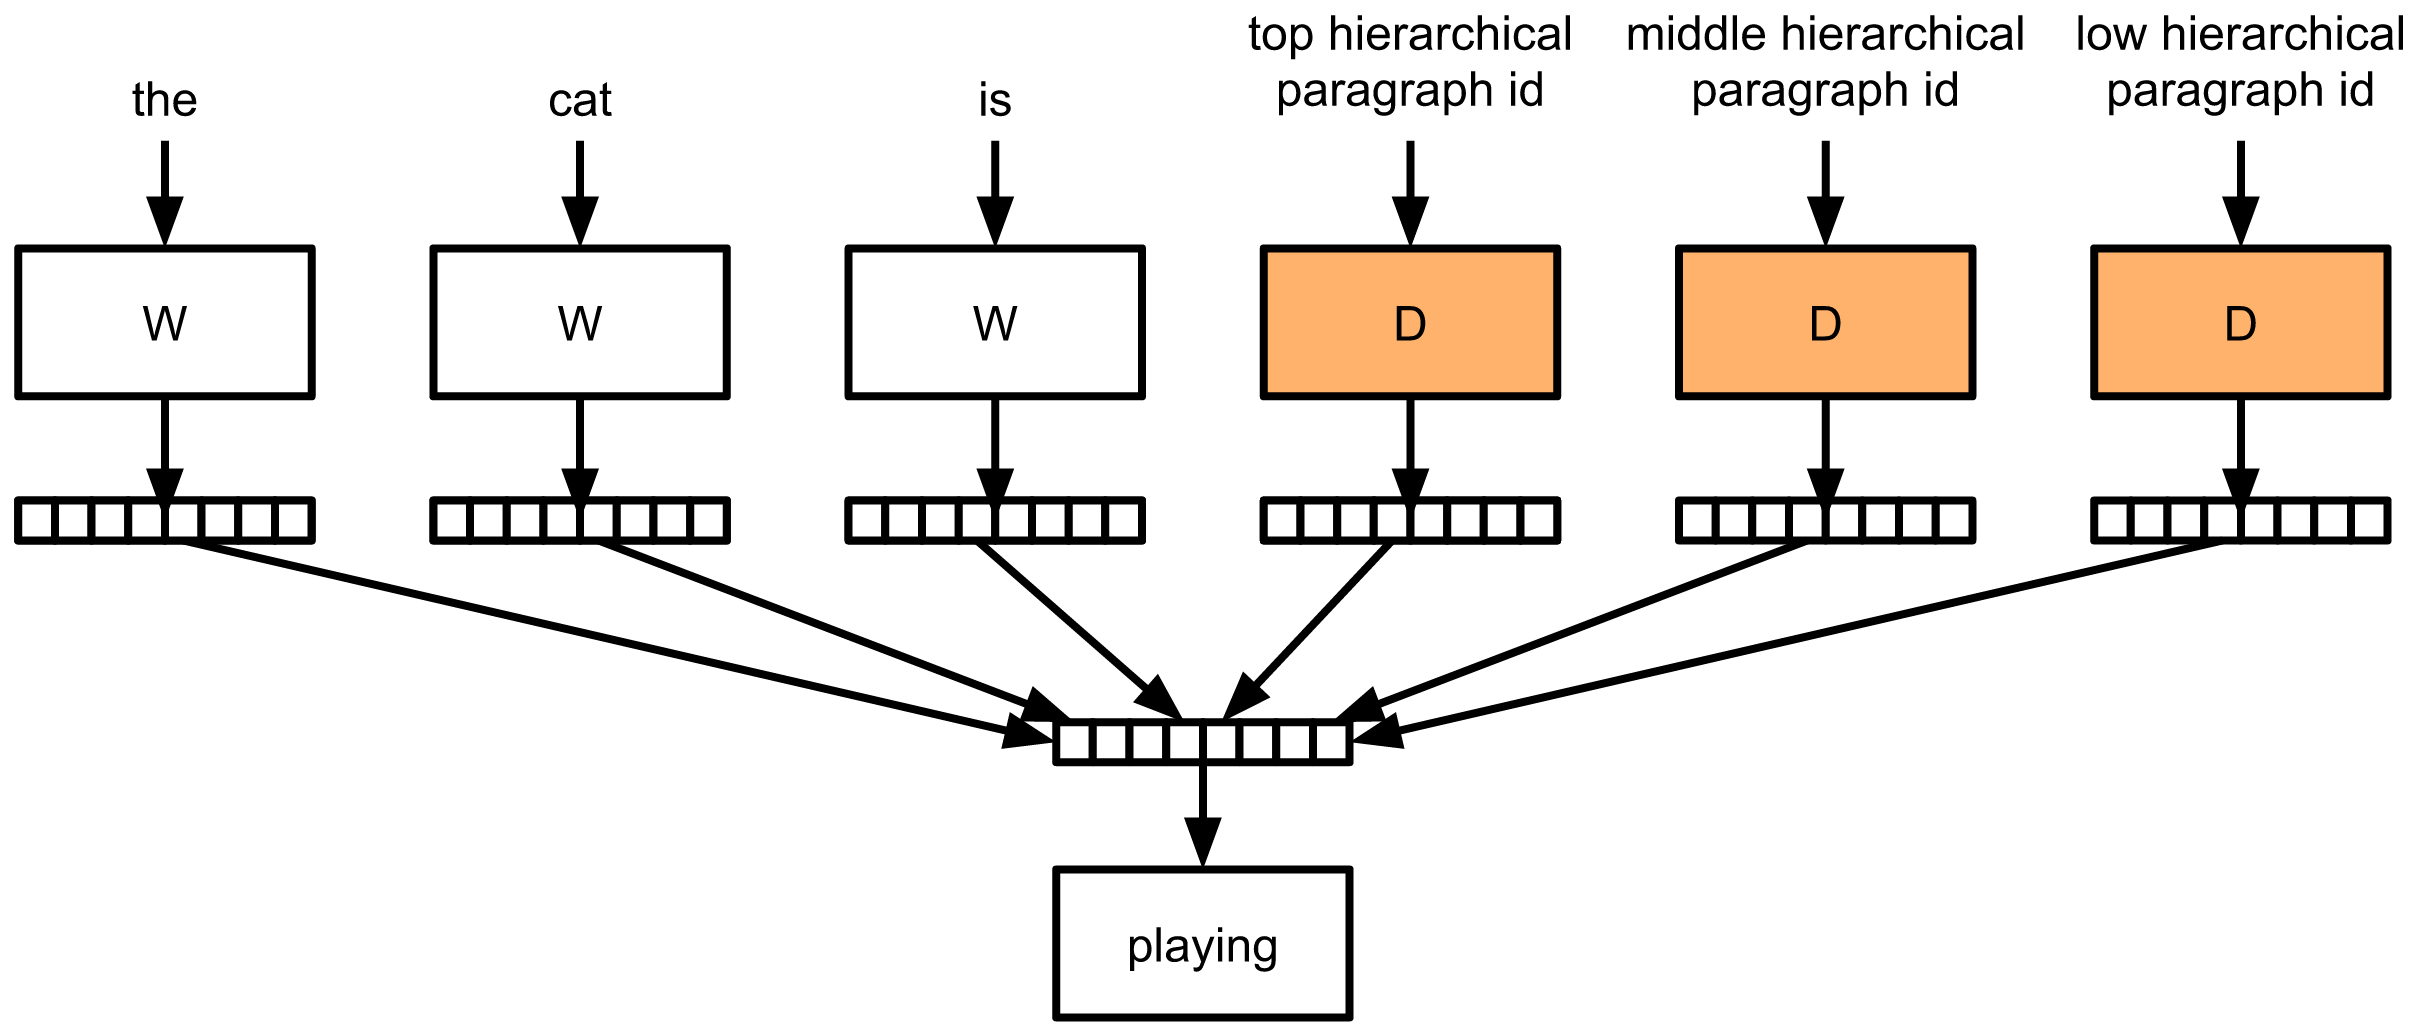
\includegraphics[width=1.0\textwidth]{4hpvs/hpv-dm.png}
	\caption{The architecture of the neural network of HPV-DM\@. Multiple HPVs contribute to the prediction of the word in the context.}
	\label{fig:4:hpv-dm}
\end{figure}

The algorithm works as follows. We split the text into multiple text blocks, according to the hierarchies we want to use. Every item in the hierarchy receives a \emph{unique HPV identifier across the whole dataset}. Next, we add each resulting text block with the HPV annotations as paragraph vectors for training. Then, we train each sentence the same way we would train it with PV-DM, but now each text block has multiple HPVs (paragraph vectors), and each HPV is shared among text blocks which have the same HPV annotation. Therefore, each HPV annotation is expected to contribute to the prediction task. As a bonus, the algorithm generates an embedding for each HPV annotation.

%todo low prio write down the algorithm

For example, when we want to use category (upwards), document (the element for which we would like to have an embedding) and sentence (downwards), we generate, for example, ``CAT-10'' for category \#10, ``DOC-2'' for document \#2, and ``DOC-2-SEN-3'' for sentence \#3 in document \#2. Next, when sentence \#3 in document \#2 belongs to the categories \#10 and \#5, we generate ``CAT-10'', ``CAT-5'', ``DOC-2'' and ``DOC-2-SEN-3'' for this sentence. When we now train the sentences in document \#2, the vector for annotation ``DOC-2'' is shared among the sentences.

\subsection{HPV-DBOW}\label{hpv-dbow}

HPV-DBOW works analogously to the HPV-DM, but it enhances the PV-DBOW algorithm instead of the PV-DM algorithm. For the implementation, the only difference is that we use PV-DBOW instead of PV-DM for training. The neural network architecture is described in Figure~\ref{fig:4:hpv-dbow}. We notice that HPVs in higher hierarchies must support more abstract and general concepts.

\begin{figure}
	\centering
	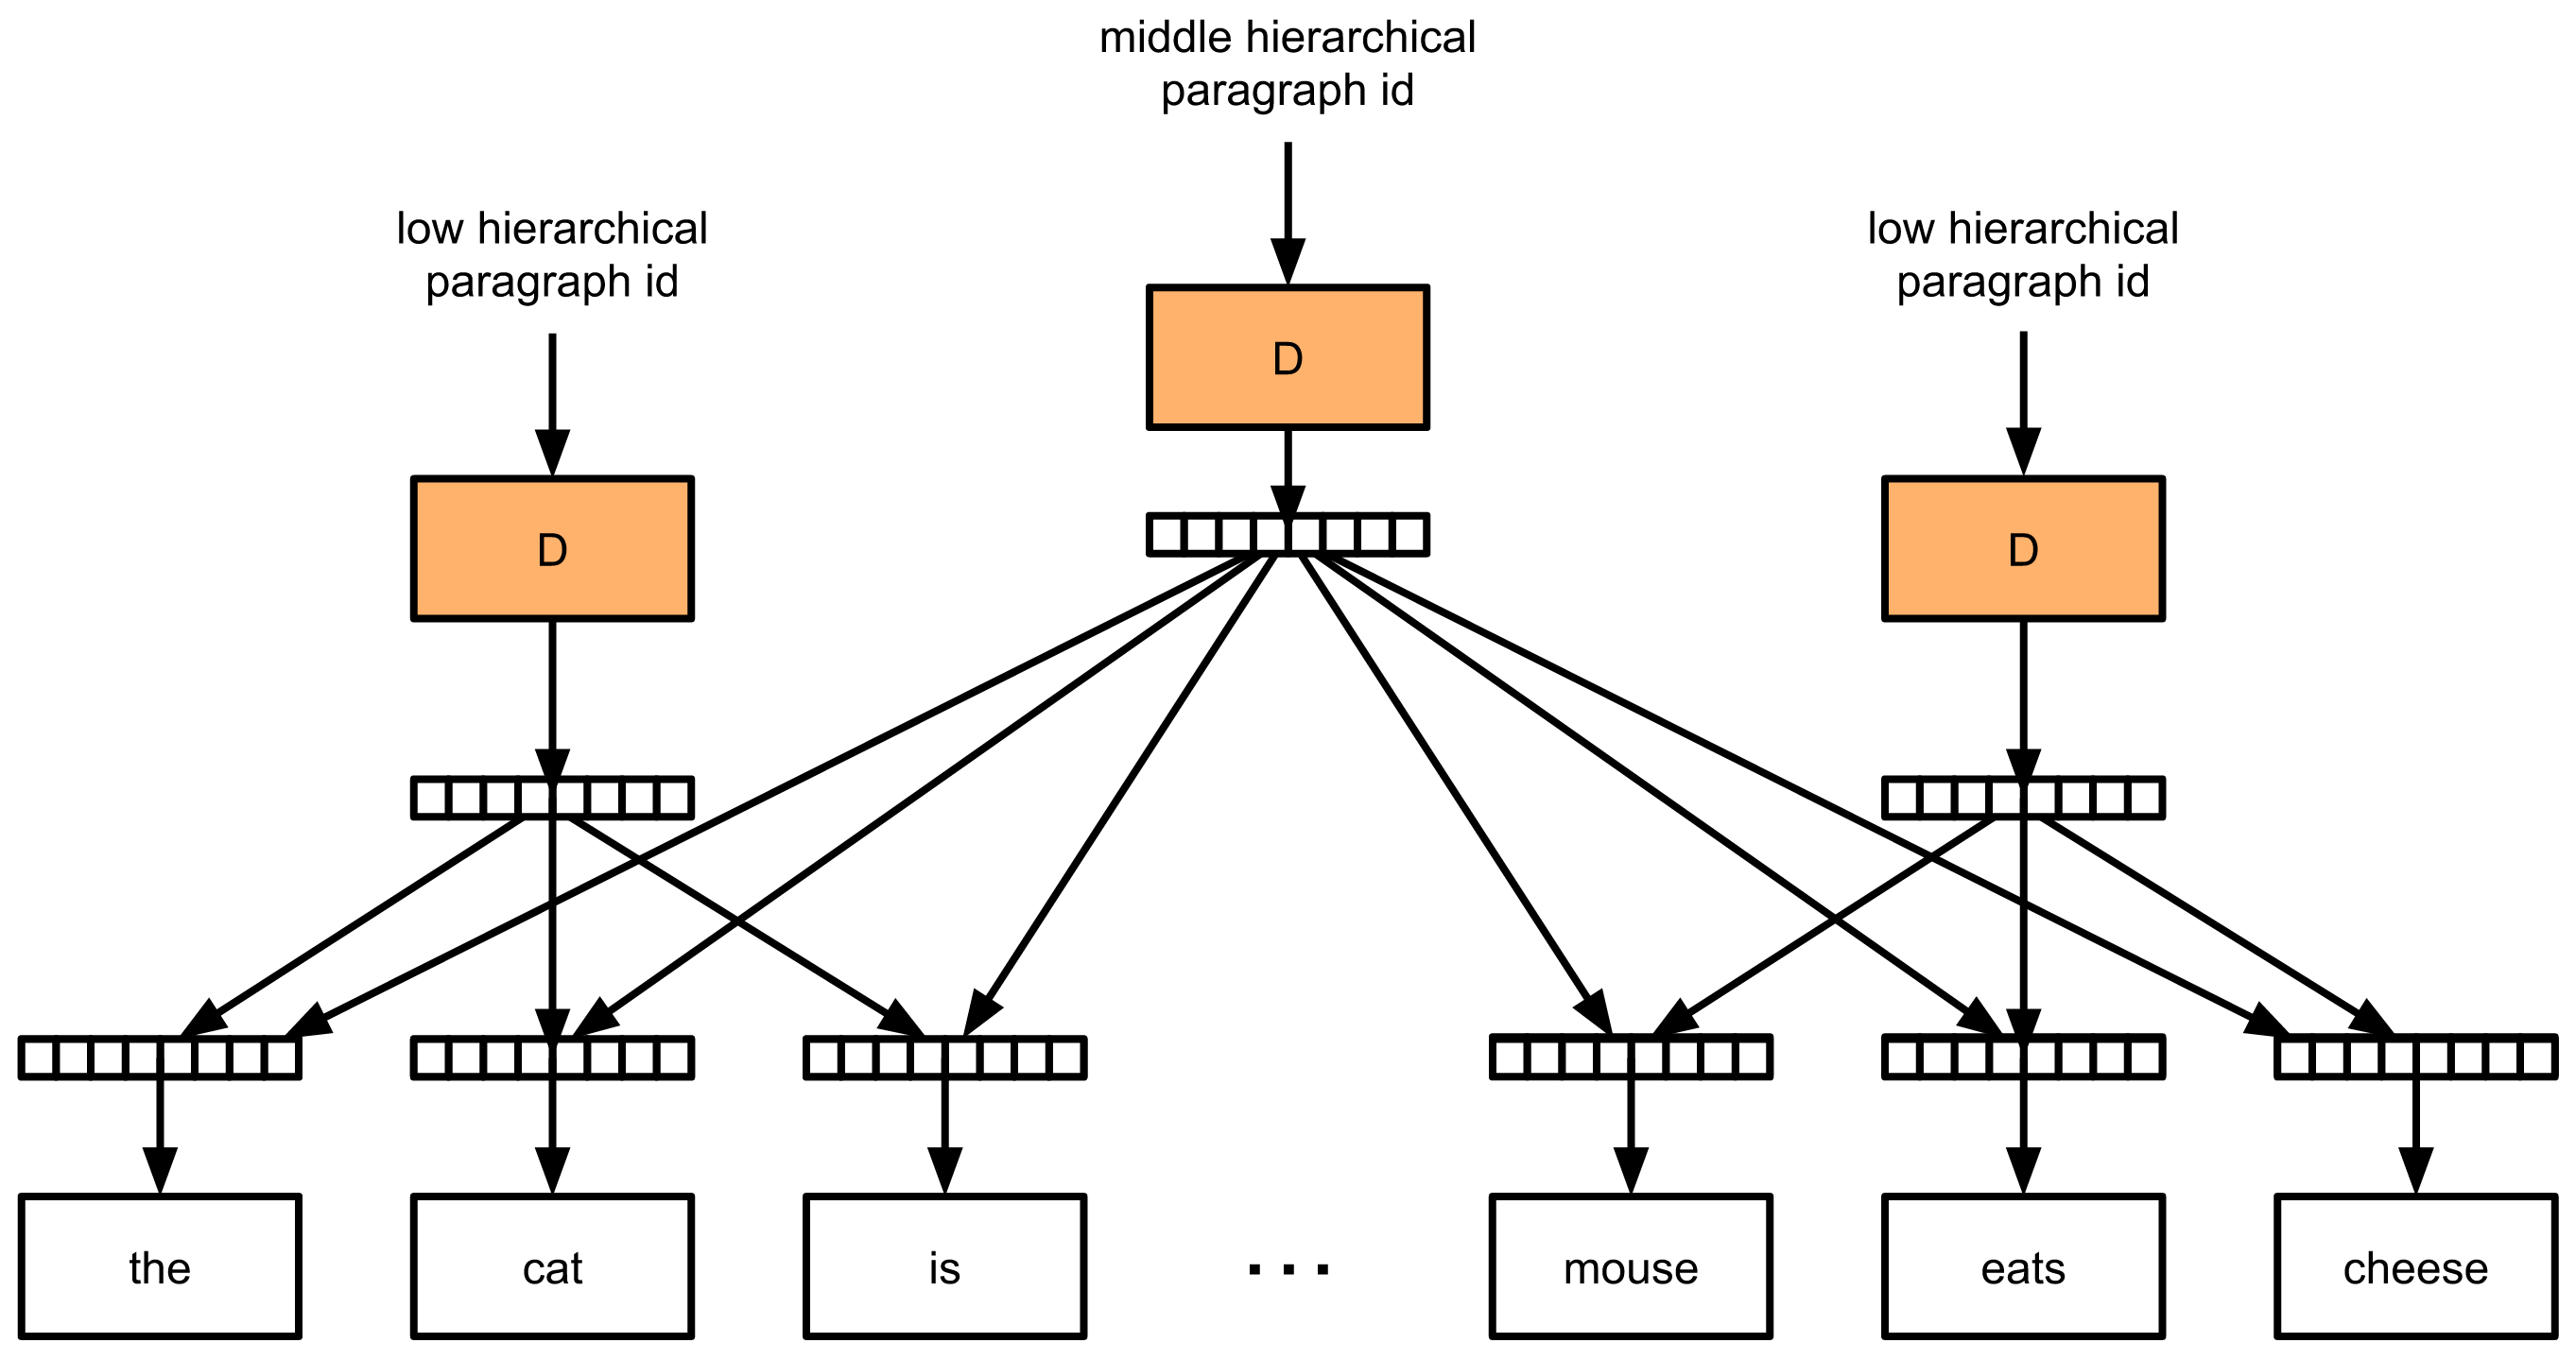
\includegraphics[width=1.0\textwidth]{4hpvs/hpv-dbow.png}
	\caption{The architecture of the neural network of HPV-DBOW\@. Every HPV predicts the context around it. HPVs in higher hierarchies represent more abstract concepts. For example, the lower HPV on the left side captures the behavior of cats, and the lower HPV on the right side captures the behavior of mice. The middle HPV must capture both concepts, which is the behavior of mammals.}
	\label{fig:4:hpv-dbow}
\end{figure}

\subsection{Parameters}\label{parameters}

Because HPV-DM and HPV-DBOW directly extend HP-DM and HP-DBOW respectively, they directly inherit the parameters from these models. However, they introduce a new parameter that dictates which hierarchies should be exploited for learning. While this parameter is limited by the data available, it is important to consider only using the ones which improve the end result, as will be illustrated later.

\section{Resources}\label{4:resources}

When using HPV, we expect to extract additional information at the cost of greater overhead. To estimate how much overhead is introduced, we will discuss how the resources required change when running HPV compared to running PV\@. Therefore, we must first understand how PV influences the resources needed.

Let us start with some definitions. $D$ is the (hierarchical) paragraph vector dimensionality, $E$ is the word vector dimensionality, $G$ is the number of unique different hierarchy elements used, $K$ is the number of paragraph vectors per document, $N$ stands for the number of documents used and $U$ is the vocabulary.

For the Word2vec model, we need to store one word vector per word, which is $E \times \dim(U)$. The paragraph vector models need to additionally store the paragraph vectors, which is $D \times K \times N$ additional memory. Finally, HPV needs to store $D \times G$ additional hierarchical paragraph vectors. Let us write down the formula for the approximate additional memory consumption.
\begin{displaymath}
\frac{D \times G}{E \times \dim(U) +D \times K \times N}
\end{displaymath}

Now, let us briefly discuss what these formulas mean by three typical examples. Let us assume $N=100'000$ documents, $Z=1'000$ average words per document, $D=E=100$ dimensions, $dim(U)=25'000$ vocabulary size, $W=20$ window size, $K=1$ paragraph vectors per document. For the first example, let us assume that we go up in the hierarchy, having 10 topics and 100 subtopics in total. This means $G=110$. In this case, only about 0.009\% additional memory is used. For the second example, assuming that we go downwards, we have 5 sentences per paragraph. This results in $G=50'000$, which means that 143\% additional memory is required. For the third example, let us assume that in addition to the sentences of the second example, there are 4 sub-sentences (in total 200'000) per sentence. Thus, $G=250'000$, which results in 714\% additionally required memory.

Because of the non-trivial optimizations of Word2vec, the runtime implications are more difficult to estimate. Thus, they are not estimated theoretically, but evaluated empirically in Chapter~\ref{experiments} instead.

\section{Research Questions}

As we have seen, HPV introduces additional model complexity. Depending on the number of implemented hierarchy layers, the model gains additional freedom. Can the neural network use this additional complexity to predict better values in the output layer? How many hierarchy layers improve the quality of the word embeddings, and which layers should be chosen? How much overhead is introduced in term of computational complexity and memory usage? Do some layers improve the learning speed of the neural network through the context sharing? We will address these questions in the Chapter~\ref{experiments}.

\chapter{Experiments}\label{experiments}

The goal of the experiments is to evaluate the word vector quality. First, we briefly describe the data, preprocessing and evaluation metrics. Next, we describe the testing environments (hardware and software). Moreover, the baseline methods are outlined. Furthermore, the implemented HPV hierarchies are described, and the possible hyperparameters will be outlined. Finally, the results will be shown.

\section{Experimental Setup and Data}\label{experimental-setup-and-data}

\subsection{IMDB Dataset}\label{imdb-dataset}

The Internet Movie Database (IMDB) dataset is a collection of movie reviews which have been written and rated by people. Each movie review consists of a text, which, in turn, consists of some sentences and has one or multiple paragraphs.

Additionally, half of the movie ratings have a rating $r \in [1,\ 10] \subseteq \mathbb{N}$, where a higher rating indicates that the reviewer likes the movie better. Furthermore, the movie ratings are divided into \emph{negative ratings} (numeric rating of 1, 2, 3 or 4) and \emph{positive ratings} (numeric rating of 7, 8, 9 or 10). \emph{Neutral ratings} with a numeric rating of 5 or 6 have been excluded from the dataset. The task is to perform sentiment analysis on the movie reviews: for a given review text, predict if the sentiment is positive or negative.

Besides the rated reviews, the other half of the reviews do not contain a rating and thus can only be used to learn the word embeddings, as we will see later. The distribution of the 100'000 movie rating can be seen in Figure~\ref{fig:5:movie-ratings-distribution}. More detailed information about the dataset can be found in~\cite{Maas2011}.

\begin{figure}
	\centering
	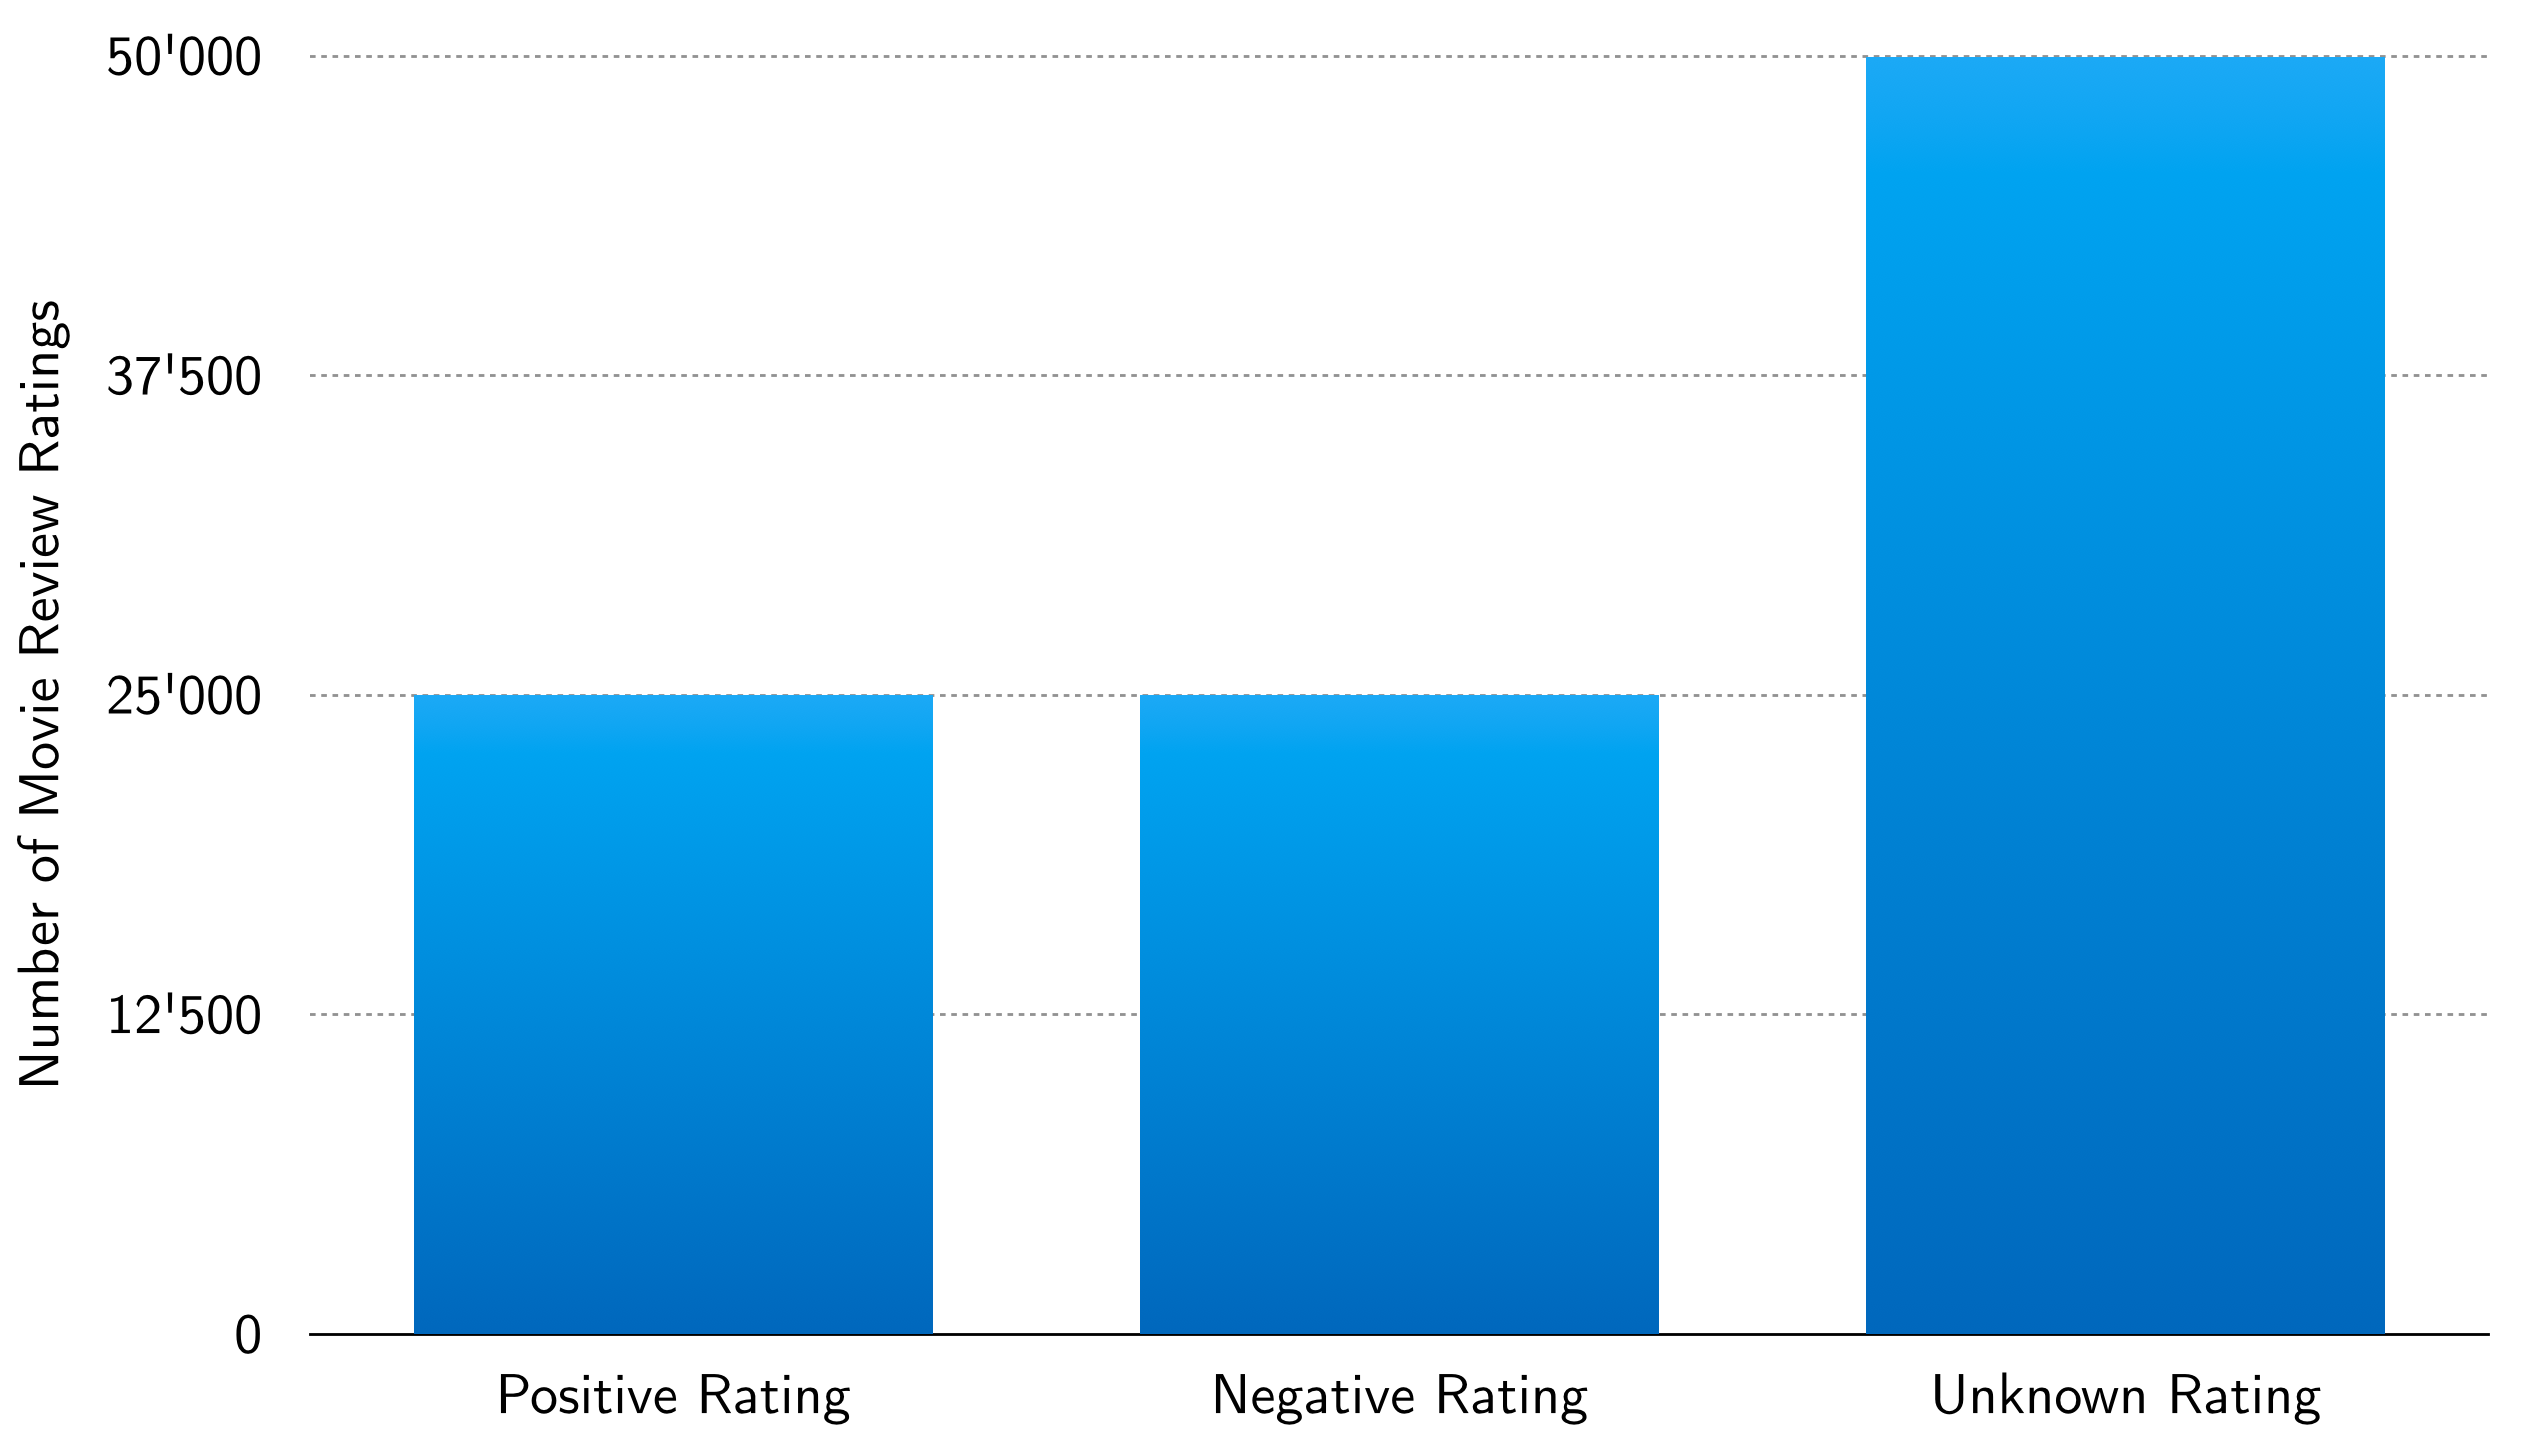
\includegraphics[width=1.0\textwidth]{5experiments/movie-ratings-distribution.png}
	\caption{The movie review ratings consist of an equal amount of positive and negative ratings. For half of the dataset, the rating is unknown.}
	\label{fig:5:movie-ratings-distribution}
\end{figure}


\subsection{Preprocessing}\label{preprocessing}

Preprocessing of text can lead to significant differences in the outcome of the results. Additionally, it can also help to reduce computational complexity, for example by removing invalid characters, which would be used as words, or by converting some similar characters to one general character. However, preprocessing is not the focus of this master thesis, and is therefore only applied limitedly.

First, different single quote symbols (for example ', ", `) are consolidated, and so are different double quote symbols. Next, frequently used HTML tags are converted to text symbols. Furthermore, common smilies are replaced by text symbols. Finally, punctuation, brackets, and commonly used special characters (for example dollar, hashtag) are replaced by text symbols. Other invalid symbols and uncommonly used characters are removed from the text. Finally, all text is converted to lowercase.

\subsection{Software}\label{software}

The original implementation by Mikolov only works for Word2vec, and would have to be extended to work with Doc2vec. Furthermore, this implementation is written in pure C, and is therefore difficult to modify, extend, and interact with.

There exist many implementations for Doc2vec. One of the fastest, if not the fastest implementation, is Gensim\footnote{\url{https://radimrehurek.com/gensim/}}. Furthermore, the implementation has a well-defined and simple interface to Python\footnote{\url{https://www.python.org/}}, and is well documented. For these reasons, Gensim was chosen as a library for the paragraph vector calculation. The exact versions are 3.4.3 for Python, and 0.12.1 for Gensim. The source code produced in the course of this thesis project can be found here\footnote{\url{https://github.com/lukaselmer/hierarchical-paragraph-vectors}}.

\subsection{Distributed Implementation}\label{distriubted-implementation}

To run a large amount of experiments and to record the results, the experiments needed to be run on a cluster. Thus, an implementation, which can distribute jobs and record results, was required. One job that consists of the parameters described below is executed on exactly one node, and is run through the whole dataset. Thus, the computation is not distributed in the traditional map-reduce way.

Running one batch of experiments works as follows: on one central server, the experiments are scheduled. Then, a client requests the parameters for one experiment to run, runs the experiment with these parameters, and submits the result to the central server. This process is executed as long as there are scheduled experiments. An overview of the architecture can be found in Figure~\ref{fig:5:architecture}.

\begin{figure}
	\centering
	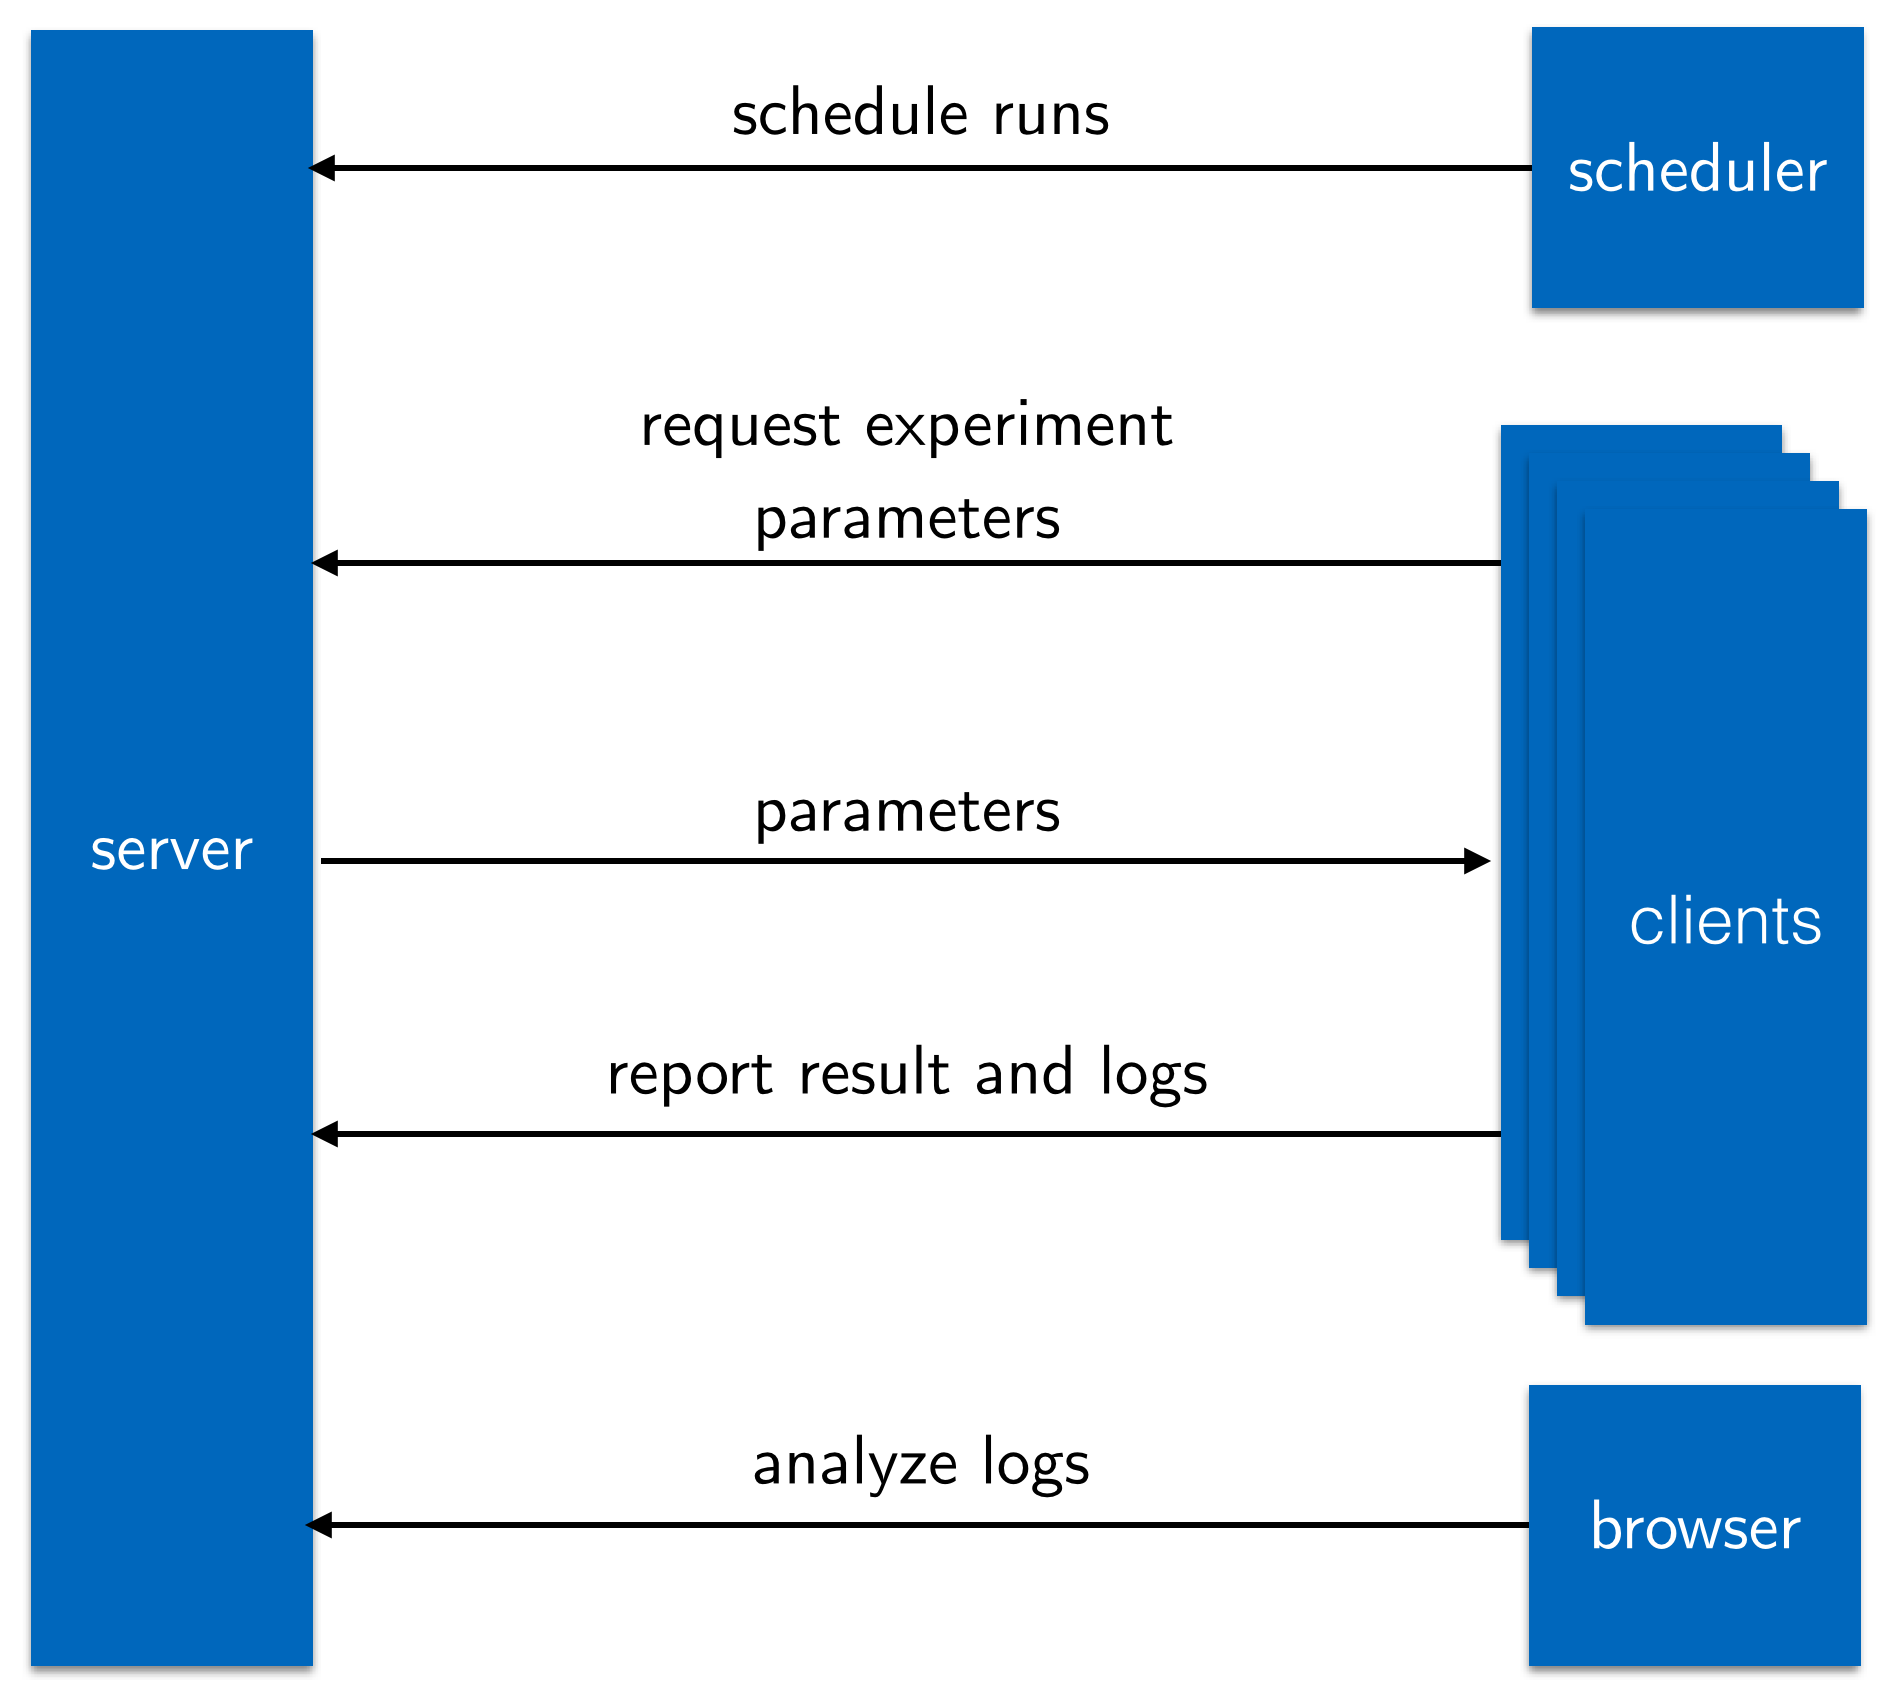
\includegraphics[width=0.7\textwidth]{5experiments/architecture.png}
	\caption{Architectural overview of the distributed implementation. The tiers communicate via HTTPS and JSON.}
	\label{fig:5:architecture}
\end{figure}

The central server is implemented in Ruby on Rails\footnote{\url{https://github.com/lukaselmer/simple-job-runner}}. In addition to the scheduling and result collection, the server also implements an interface to analyze the results and to generate charts. The client is implemented in Python, see~\ref{software}. Multiple clients request, run and submit experiments concurrently.

\subsection{Hardware}\label{hardware}

The software was developed on an ``Apple MacBook Pro, Core i7 2.8 (I7-4980HQ), 15-Inch, Mid-2014, Dual Graphics'', model id ``MacBookPro11,3''\footnote{\url{http://www.everymac.com/systems/apple/macbook_pro/specs/macbook-pro-core-i7-2.8-15-dual-graphics-mid-2014-retina-display-specs.html}}. Also, the performance tests in~\ref{5:execution-speed-and-memory-usage} have been conducted on this laptop. The operating system of the laptop was OS X Yosemite 10.10.5.

The restricted and unrestricted best configuration experiments in~\ref{5:accuracy} have been executed on 8 nodes of the DCO cluster at ETH\@. Each machine has 16 physical cores and 128 GB of physical RAM\@. The operating system of the servers was Fedora 21\footnote{\url{https://getfedora.org/}}.

\section{Evaluation Metrics}\label{evaluation-metrics}

Recall that the dataset is balanced between positive and negative ratings. Therefore, a random estimator would guess the sentiment of 50\% of the ratings correctly. The balanced dataset allows us to use accuracy as the first evaluation metric. We use the following definition to calculate the mean accuracy from the predicted reviews $R$.
\begin{displaymath}
\text{accuracy} = \frac{1}{\dim(R)} \sum_{r \in R} \begin{dcases*}
1& when $r_{\text{predicted sentiment}}$ = $r_{\text{actual sentiment}}$\\
0& otherwise
\end{dcases*}
\end{displaymath}
Note that this is a binary classification task.

The second and third evaluation metrics are training speed (computational complexity) and memory footprint which are measured empirically. The training speed is calculated by measuring the time from starting one training epoch until the training epoch has ended. Here, it is important to note that during the test, only one active program is being run on the machine, and no other computationally intensive programs are being run in the background. The memory footprint is measured by the size of a file to which the model is serialized.

\section{Baseline Methods}\label{baseline-methods}

There are two methods which draw a baseline to compare HPV to. The first baseline is to generate the word embeddings by using the commonly used term frequency - inverse document frequency (TF--IDF) method \cite{Rajaraman2011}. For the TF--IDF vectors, the features are ordered by term frequency across the corpus, and only the top $n$ features are used to get a low-dimensional vector. More details about the implementation can be found in \ref{appendix:tf-idf}.

The second baseline method is the standard implementation of Doc2vec provided by Gensim. As we will see, the same hyperparameters are used for the baseline and the HPV enhanced implementation.

Both baseline methods use the same classifier as the HPV implementations, which is a support vector classifier (SVC), see Table ~\ref{tab:parameters}.

\section{Implemented HPV Hierarchies}\label{implemented-hpv-hierarchies}

As we have seen before, there are two directions from which hierarchies can be obtained (upwards and downwards). Let us first investigate the upwards direction and thereafter continue with the downwards direction.

\begin{table}
	\centering
	\caption{Overview of the implemented hierarchies.}
	\label{tab:implemented-hpv-hierarchies}
	\begin{tabular}{ll}
		\toprule
		\emph{Abbreviation}& \emph{Hierarchies}\tabularnewline
		\midrule
		NO-HPV& None\tabularnewline
		HPV-TOP& Topics\tabularnewline
		HPV-TOP-PAR& Topics, Paragraphs\tabularnewline
		HPV-TOP-PAR-SENT& Topics, Paragraphs, Sentences\tabularnewline
		HPV-PAR& Paragraphs\tabularnewline
		HPV-PAR-SENT& Paragraphs, Sentences\tabularnewline
		HPV-PAR-SENT-SUB& Paragraphs, Sentences, Sub-sentences\tabularnewline
		HPV-PAR-SENT-SUBNV& \begin{tabular}[x]{@{}l@{}}Paragraphs, Sentences, Sub-sentences (but\\without training the sub-sentence vectors)\end{tabular}\tabularnewline
		\bottomrule
	\end{tabular}
\end{table}

The IMDB movie rating dataset has natural hierarchies (for example the movie category, actors, year), but unfortunately, these hierarchies are not annotated in the dataset. Therefore, we use LDA to extract a synthetic hierarchy. We extract 20 topics from the data by running LDA for 20 iterations. Then we assign the two most corresponding topics, which have a probability greater 25\% to occur per movie review. This topic is then stored as a special word. Runs using these topics are labeled as ``TOP''.

Now let us turn our attention to the ``downwards'' hierarchies. First, we use paragraphs as a hierarchy, which we denote as ``PAR''. Next, we parse the sentences, denoted as ``SENT''. Finally, ``SUB'' stands for sub-sentences, and ``SUBNV'' stands for sub-sentence splitting, but not learning a vector per sub-sentence. Finally, the hierarchies are combined. An overview can be found in Table~\ref{tab:implemented-hpv-hierarchies}. When we preprocess and split up the dataset, we extract the following number of elements displayed in Table~\ref{tab:5:extracted-elements}. The exact implementation of the splitting is described in~\ref{appendix:hierarchy-splitting}.

\begin{table}
	\centering
	\caption{The number of extracted elements from the data after preprocessing and splitting considering the HPV Hierarchies.}
	\label{tab:5:extracted-elements}
	\begin{tabular}{lr}
		\toprule
		\emph{Variable}& \emph{Value}\tabularnewline
		\midrule
		Topics& 20\tabularnewline
		Documents& 100'000\tabularnewline
		Paragraph Vectors per Document& 1\tabularnewline
		Vocabulary Size& 185'957\tabularnewline
		Total Words& 27'527'432\tabularnewline
		Average Words per Document& 275\tabularnewline
		Paragraphs& 303'448\tabularnewline
		Sentences& 1'613'409\tabularnewline
		Sub-sentences& 3'061'360\tabularnewline
		\bottomrule
	\end{tabular}
\end{table}


\section{Hyperparameters}\label{hyperparameters}

Hyperparameter search is known to be a key challenge in applied machine learning. There are known procedures, such as grid search, but in practice, this problem is more difficult than it is in theory. The climax of this challenge is the explosive count of combinations of hyperparameters, where each combination could potentially outperform a very distant other combination, making it a non-convex problem. What makes it even more difficult is that it takes much time for one combination to evaluate, which we will see later.

In Table~\ref{tab:parameters}, the values of the most important hyperparameters are stated. Furthermore, the ranges, in which these values have been searched in, are described.

\subsection{Epochs}

The number of iterations the dataset is processed. For each iteration, the order of the texts is shuffled.

\subsection{HPV Hierarchies}

The hierarchies which should be exploited, see~\ref{implemented-hpv-hierarchies}.

\subsection{Word Vector Dimensionality}

The dimensionality of the word vectors and paragraph vectors for HPV-DM and HPV-DBOW \emph{each}.

\subsection{Window Size}

The window size in each direction (left and right), see Figure~\ref{fig:3:sliding-window}.

\subsection{Negative Sampling}

The number of negative samples per positive sample.

\subsection{Frequent Word Downsampling HPV-DM}

Threshold to downsample frequent words for HPV-DM\@.

\subsection{Frequent Word Downsampling HPV-DBOW}

Threshold to downsample frequent words for HPV-DBOW\@.

\subsection{Learning Rate Type}

The function that shows how to decrease the learning rate. Exponential (exp) or linear (lin). More details can be found in the Appendix~\ref{appendix:learning-rate-type}.

\subsection{Classifier}

The classifier used to learn (from the word embeddings and given ratings) to predict the rating (for new word embeddings / the test set). Additionally, different classifiers have different hyperparameters. Different classifiers have been tried. 

\begin{description}
	\item[RBF] Radial basis function approximation using the Nystroem method\footnote{\url{http://scikit-learn.org/stable/auto_examples/plot_kernel_approximation.html}}.
	\item[LOG1] Logistic regression using scikit-learn\footnote{\url{http://scikit-learn.org/stable/modules/generated/sklearn.linear_model.LogisticRegressionCV.html}}.
	\item[LOG2] Logistic regression using statsmodels\footnote{\url{http://statsmodels.sourceforge.net/0.6.0/generated/statsmodels.discrete.discrete_model.Logit.html}}.
	\item[SVC] Support vector classifier using scikit-learn\footnote{\url{http://scikit-learn.org/stable/modules/generated/sklearn.svm.LinearSVC.html}}.
	\item[NN] A neural network classifier using scikit-neuralnetwork\footnote{\url{https://github.com/aigamedev/scikit-neuralnetwork}}.
\end{description}

\begin{table}
	\centering
	\caption{The value ranges and the values chosen from the most important hyperparameters. The step sizes for the value ranges were exponential at first, and after a reasonable hyperparameter combination was found, they were linear for fine-tuning.}
	\label{tab:parameters}
	\begin{tabular}{llr}
		\toprule
		\emph{Name}& \emph{Range / Options}& \emph{Best / Chosen}\tabularnewline
		\midrule
		Epochs& $[5,\ 50]$& 20\tabularnewline
		HPV Hierarchies& \begin{tabular}[x]{@{}l@{}}TOP, PAR, SENT,\\SUB, SUBNV\end{tabular}& TOP\tabularnewline
		Word Vector Dimensionality& $[16,\ 2000]$& 200, 48\tabularnewline
		Window Size& $[5,\ 25]$& 10\tabularnewline
		Negative Sampling& $[5,\ 30]$& 25\tabularnewline
		\begin{tabular}[x]{@{}l@{}}Frequent Word Downsampling\\HPV-DM\end{tabular}& $[10^{-10},\ 0.1]$& $10^{-5}$\tabularnewline
		\begin{tabular}[x]{@{}l@{}}Frequent Word Downsampling\\HPV-DBOW\end{tabular}& $[10^{-10},\ 0.1]$& $10^{-3}$\tabularnewline
		Learning Rate Type& exp, lin& exp\tabularnewline
		Classifier& RBF, LOG1/2, SVC& SVC\tabularnewline
		\bottomrule
	\end{tabular}
\end{table}

\section{Results}\label{results}

For this master thesis, more than 23'000 runs have been recorded systematically. Before that, the algorithm and framework have been developed, and the hyperparameters which should vary have been defined. Then, the first 10'000 runs have been used to find the best hyperparameters for NO-HPV and HPV-PAR-SENT-SUB using grid search. For the next 2'000 runs, HPV-PAR-SENT-SUBNV and HPV-PAR-SENT have been compared against NO-HPV and HPV-PAR-SENT-SUB\@. During the next 3'000 runs, the TF--IDF baseline has been evaluated, also in combination with NO-HPV, HPV-PAR-SENT-SUB, HPV-SUBNV and HPV-SENT-SUB\@. Furthermore, HPV-TOP and HPV-TOP-PAR-SEN were implemented, and 2'000 runs were conducted to compare them against NO-HPV\@. Moreover, HPV-TOP-PAR and HPV-PAR were implemented and compared against NO-HPV for the next 2'000 runs. Finally, the best performing configurations have been chosen to perform significance tests by executing multiple runs using the same configuration for the next 3'000 runs, before running the TF--IDF baseline for another 1'000 runs.

In this section, we will first investigate the accuracy. After this, we will turn our attention to the runtime and memory usage.

\subsection{Accuracy}\label{5:accuracy}

In this subsection, we will compare the accuracy of the HPV implementations to each other and to the baselines Doc2vec and TF--IDF\@. First, TF--IDF is compared to Doc2vec. Next, the different HPV implementations are compared to each other. Finally, the best configurations are compared to the Doc2vec baseline NO-HPV\@.

\subsubsection{Term Frequency - Inverse Document Frequency (TF--IDF)}

As we can see in Figure~\ref{fig:5:results-tfidf}, the accuracy increases when we increase the TF--IDF dimensionality. We also notice a linear increase between the 100 and 600 dimensions. When increasing the dimensionality further, the accuracy flattens out. The best accuracy of 87.9\% for TF--IDF was measured with a dimensionality of 2700. When increasing the dimensionality even further up to 4000 dimensions, the accuracy stayed between 87.5\% and 87.9\%.

\begin{figure}
	\centering
	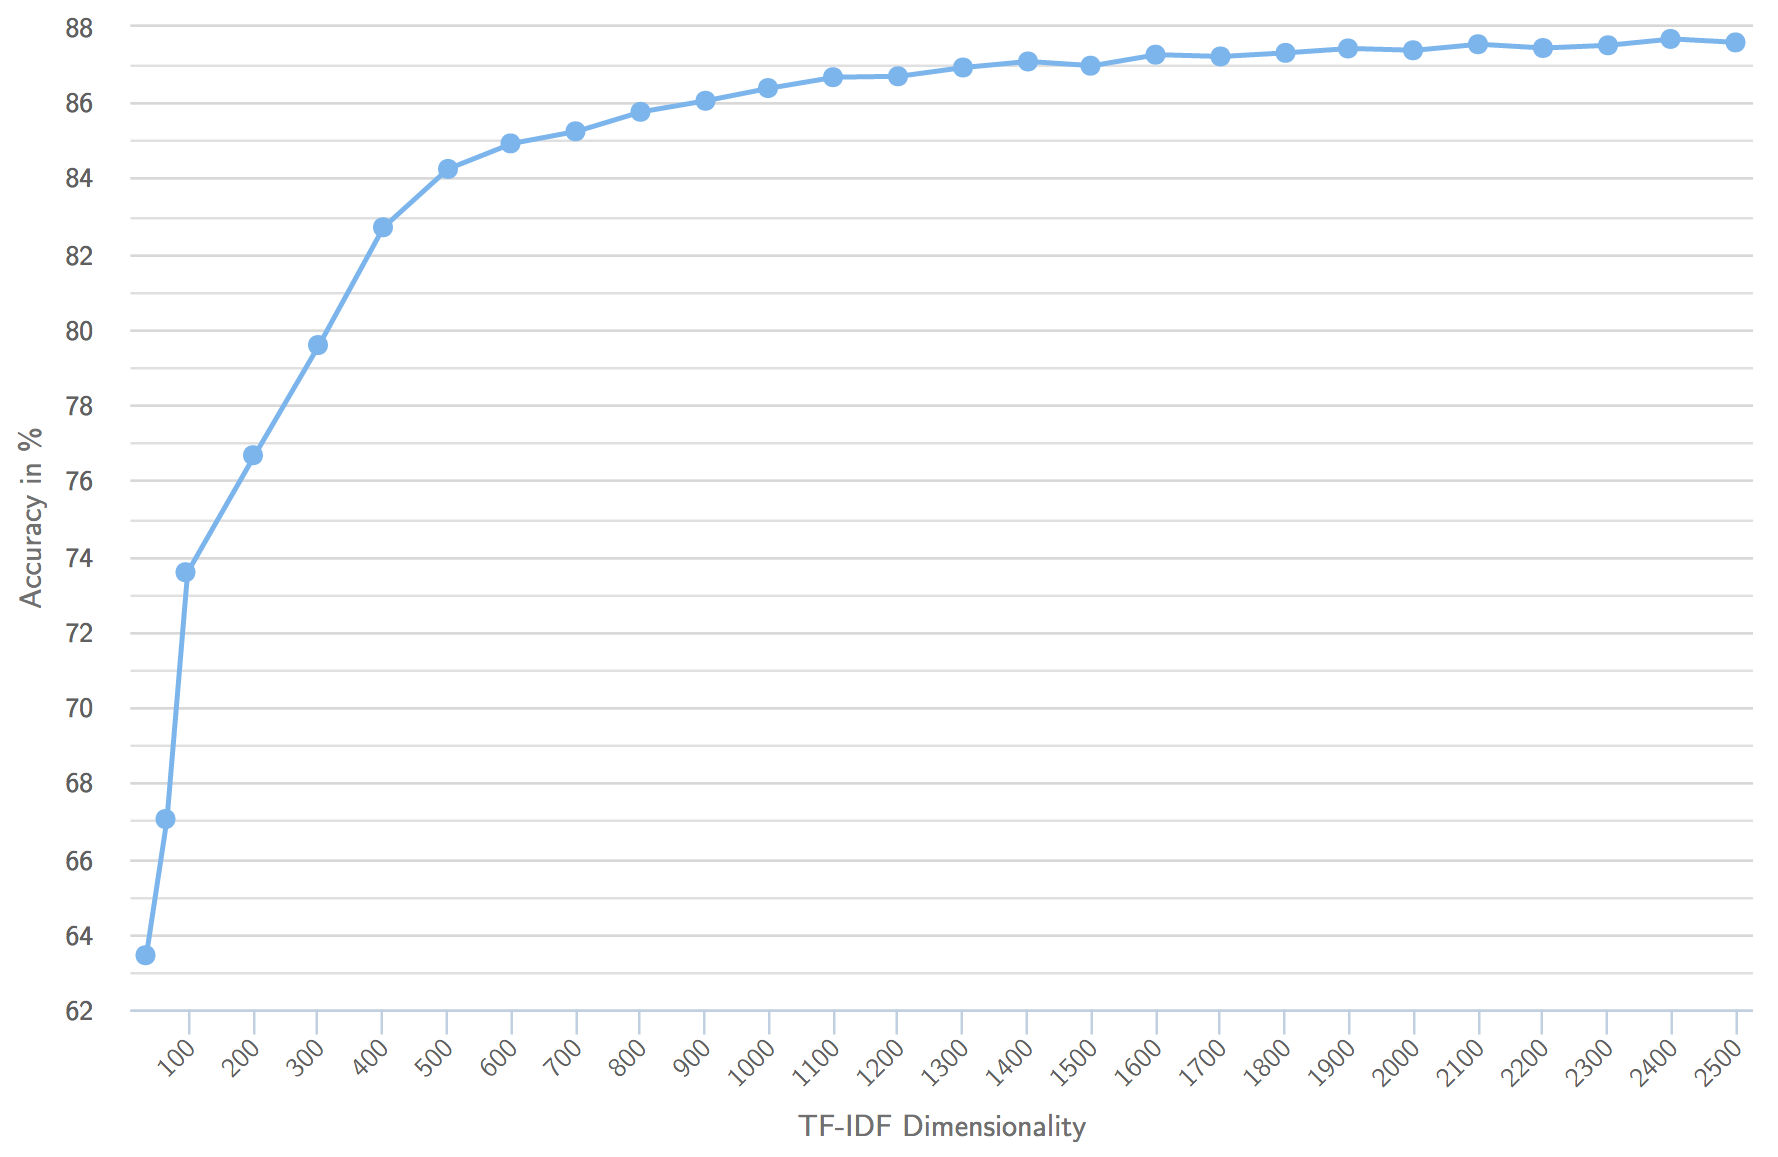
\includegraphics[width=1.0\textwidth]{5experiments/results-tfidf}
	\caption{The accuracy increases when the TF--IDF dimensionality is increased. }
	\label{fig:5:results-tfidf}
\end{figure}

When we compare the result to the values after 10 epochs of Doc2vec with 48 dimensions, see Figure~\ref{fig:5:epochs-vs-accuracy-48}, we notice that the accuracy is approximately 88.5\% in the Doc2vec case (using a total of 96 dimensions), compared to only 73.5\% accuracy in the TF--IDF case (using 96 dimensions). This means that Doc2vec outperforms TF--IDF by a substantial margin when using low-dimensional vectors.

Let us now compare TF--IDF to Doc2vec with 200 dimensions, see Figure~\ref{fig:5:epochs-vs-accuracy-200}. The accuracy for Doc2vec is approximately 90\% after multiple epochs. When we compare this to the TF--IDF score using 400 dimensions, we find an accuracy of 82.7\%. Again, Doc2vec beats the TF--IDF baseline by a considerable margin.

\subsubsection{Different HPV Implementations}

To compare the different HPV implementations against each other, the hyperparameters described in Table~\ref{tab:parameters} have been used. Because some HPV implementations clearly outperformed other implementations in multiple different configurations, instead of using multiple runs and taking the average accuracy, only one run per implementation has been conducted with this configuration. Furthermore, some HPV implementations have a slow execution speed, as we will see in~\ref{5:execution-speed-and-memory-usage}. Therefore, the additional computational cost to run multiple experiments for HPV implementations, which performed poorly, was not justified.

\begin{figure}
	\centering
	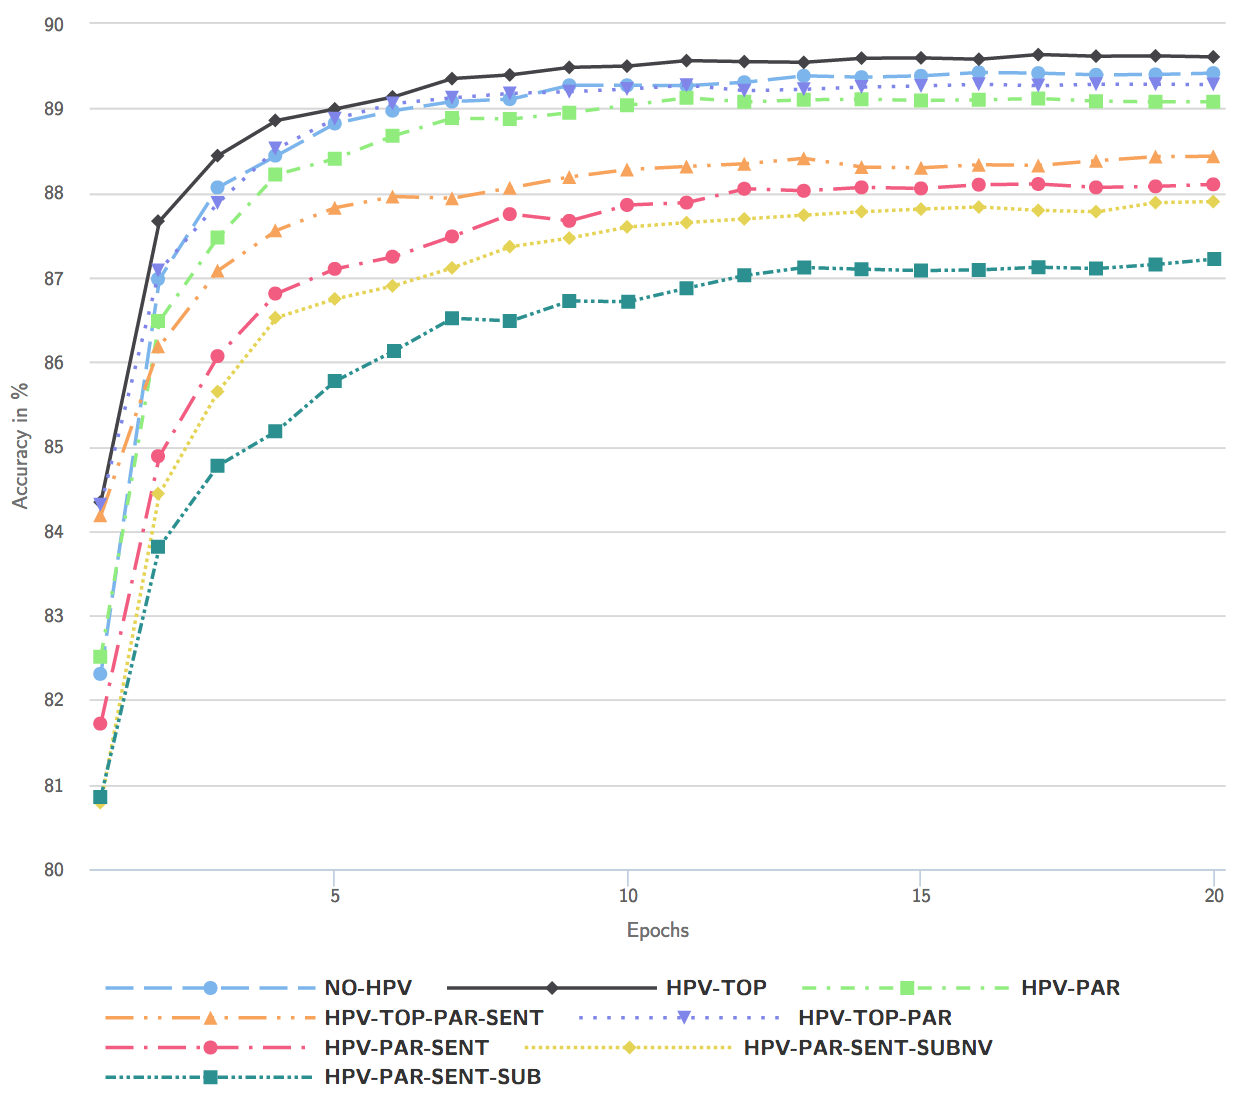
\includegraphics[width=1.0\textwidth]{5experiments/hpv-implementations}
	\caption{The accuracy increases when increasing the epochs for every HPV implementation, using a word vector dimensionality of 48. TOP boosts the accuracy significantly in the beginning. Low hierarchies do not increase the accuracy.}
	\label{fig:5:hpv-implementations}
\end{figure}

Let us now compare the different HPV implementations in Figure~\ref{fig:5:hpv-implementations}. First, we notice that after one epoch, all HPV implementations using the topic (TOP) as a hierarchy significantly outperform NO-HPV by about 2\%. Also, HPV-TOP outperforms NO-HPV here. However, this gap is not significant for all epochs, which we will see later on. Next, we notice that the more we move down in the hierarchies, the worse the accuracy develops. For example, when using paragraphs, sentences and sub-sentences, the model performs significantly worse than NO-HPV\@. Finally, when combining the topic with the lower hierarchies, the topic seems to boost the accuracy throughout all epochs, and the additional hierarchies prevent a strong increase in accuracy compared to NO-HPV\@.

The best HPV implementations from this comparison (NO-HPV, HPV-TOP, HPV-PAR) are compared in more detail in the next two subsections. HPV-TOP-PAR is left out for this comparison, because it is a combination of HPV-TOP and HPV-PAR, which both are compared against each other in the next subsections.

\subsubsection{Unrestricted Best Configuration}\label{unrestricted-best-configuration}

To compare the accuracy of the best HPV implementations to NO-HPV, the best two configurations have been chosen. The first configuration is unrestricted and thus can use an arbitrary word vector dimensionality. It uses a word vector dimensionality of 200 and the hyperparameters described in Table~\ref{tab:parameters}. The experiment has been repeated for 30 times with random initializations. Because these results represent the most important results of the empirical evaluation, significance tests have been conducted. We are using a wilcoxon signed rank test, and our hypothesis is that HPV-TOP outperforms NO-HPV, which makes it a directional test. We use a level of significance of 0.025, which corresponds to a minimum z-score of 1.960\footnote{\url{http://vassarstats.net/textbook/ch12a.html}}.

\begin{figure}
	\centering
	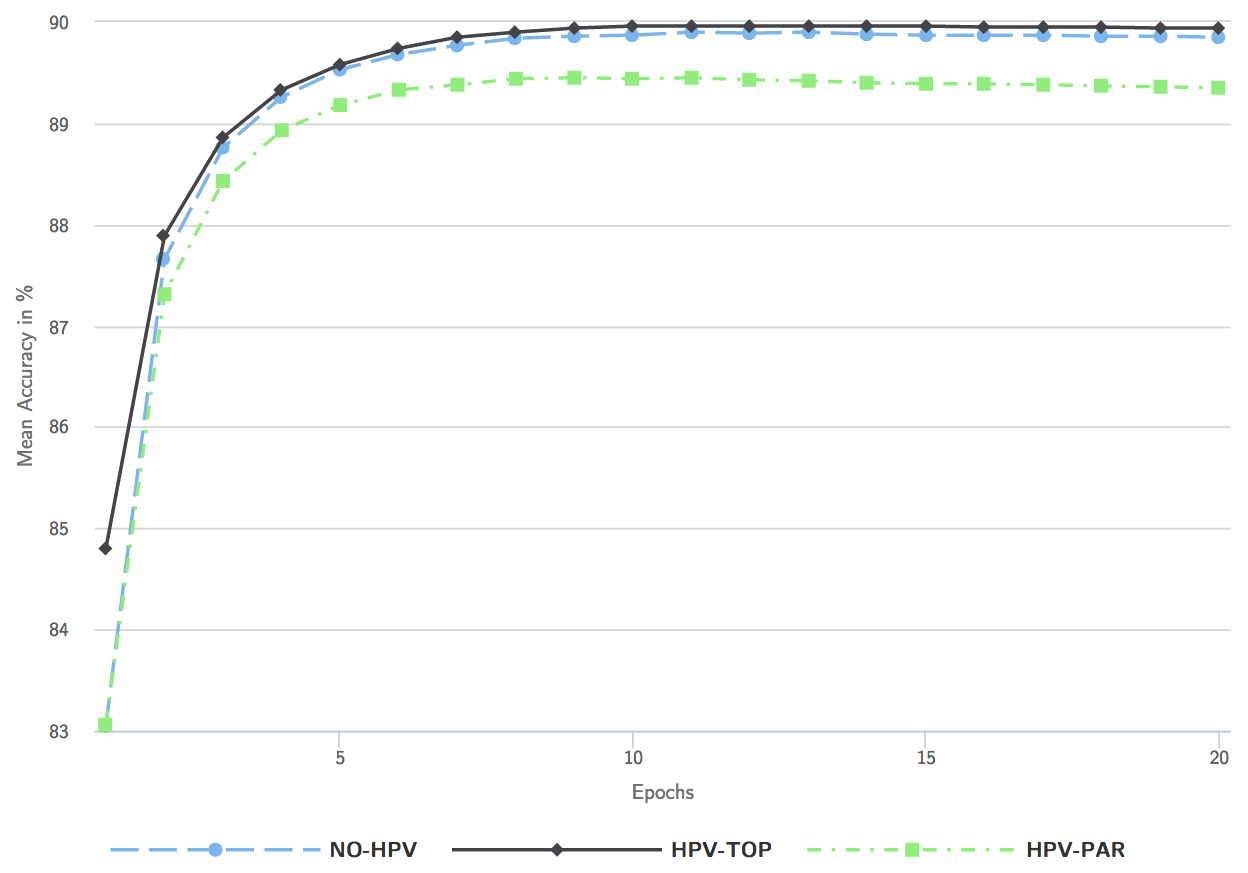
\includegraphics[width=1.0\textwidth]{5experiments/epochs-vs-accuracy-200.png}
	\caption{The mean accuracy of 30 experiments when increasing the epochs for the best configuration, using a word vector dimensionality of 200.}
	\label{fig:5:epochs-vs-accuracy-200}
\end{figure}

As we can see in Figure~\ref{fig:5:epochs-vs-accuracy-200} and Table~\ref{tab:5:epochs-vs-accuracy-200}, HPV-TOP clearly outperforms NO-HPV when only one epoch is run. When increasing the epochs, the accuracy of the prediction increases significantly for both of these implementations. HPV-TOP outperforms NO-HPV slightly by only about 0.1\%. We also notice that we reach a plateau after about 9 epochs, after which the accuracy only fluctuates marginally.

When we compare HPV-PAR to NO-HPV, we notice that after only one epoch of training, they perform very similarly. However, as the epochs progress, HPV-PAR loses steam and cannot increase the accuracy as much as NO-HPV can. Thus, NO-HPV and HPV-TOP clearly outperform HPV-PAR\@.

\begin{table}
	\centering
	\caption{The data displayed in Figure~\ref{fig:5:epochs-vs-accuracy-200}, which is the unrestricted best configuration, using word vector dimensionality of 200. The values, where HPV-TOP outperforms NO-HPV with a level of significance of 0.025, are marked with a *.}
	\label{tab:5:epochs-vs-accuracy-200}
	\begin{tabular}{lrrr}
		\toprule
		& \multicolumn{3}{c}{\emph{Accuracy [\%]}}\tabularnewline
		\emph{Epoch}& \emph{HPV-NO}& \emph{HPV-TOP}& \emph{HPV-PAR}\tabularnewline
		\midrule
		1& 83.05& *84.8& 83.06\tabularnewline
		2& 87.66& *87.89& 87.31\tabularnewline
		3& 88.76& *88.86& 88.43\tabularnewline
		4& 89.26& *89.33& 88.93\tabularnewline
		5& 89.53& 89.58& 89.18\tabularnewline
		6& 89.68& *89.74& 89.33\tabularnewline
		7& 89.77& *89.85& 89.38\tabularnewline
		8& 89.84& *89.9& 89.44\tabularnewline
		9& 89.86& *89.94& 89.45\tabularnewline
		10& 89.87& *89.96& 89.44\tabularnewline
		11& 89.9& *89.96& 89.45\tabularnewline
		12& 89.89& *89.96& 89.43\tabularnewline
		13& 89.9& 89.96& 89.42\tabularnewline
		14& 89.88& *89.96& 89.4\tabularnewline
		15& 89.87& *89.96& 89.39\tabularnewline
		16& 89.87& *89.95& 89.39\tabularnewline
		17& 89.87& *89.95& 89.38\tabularnewline
		18& 89.86& *89.95& 89.37\tabularnewline
		19& 89.86& 89.94& 89.36\tabularnewline
		20& 89.85& *89.94& 89.35\tabularnewline
		\bottomrule
	\end{tabular}
\end{table}


\subsubsection{Restricted Best Configuration}\label{restricted-best-configuration}

The second best configuration is restricted to use a low word vector dimensionality of 48 dimensions for HPV-DM and HPV-DBOW \emph{each}. For the significance tests, we apply the same strategy as in the best unrestricted configuration above, using 30 experiments with random initializations, a 0.025 level of significance, and the hypothesis that HPV-TOP outperforms NO-HPV\@.

\begin{figure}
	\centering
	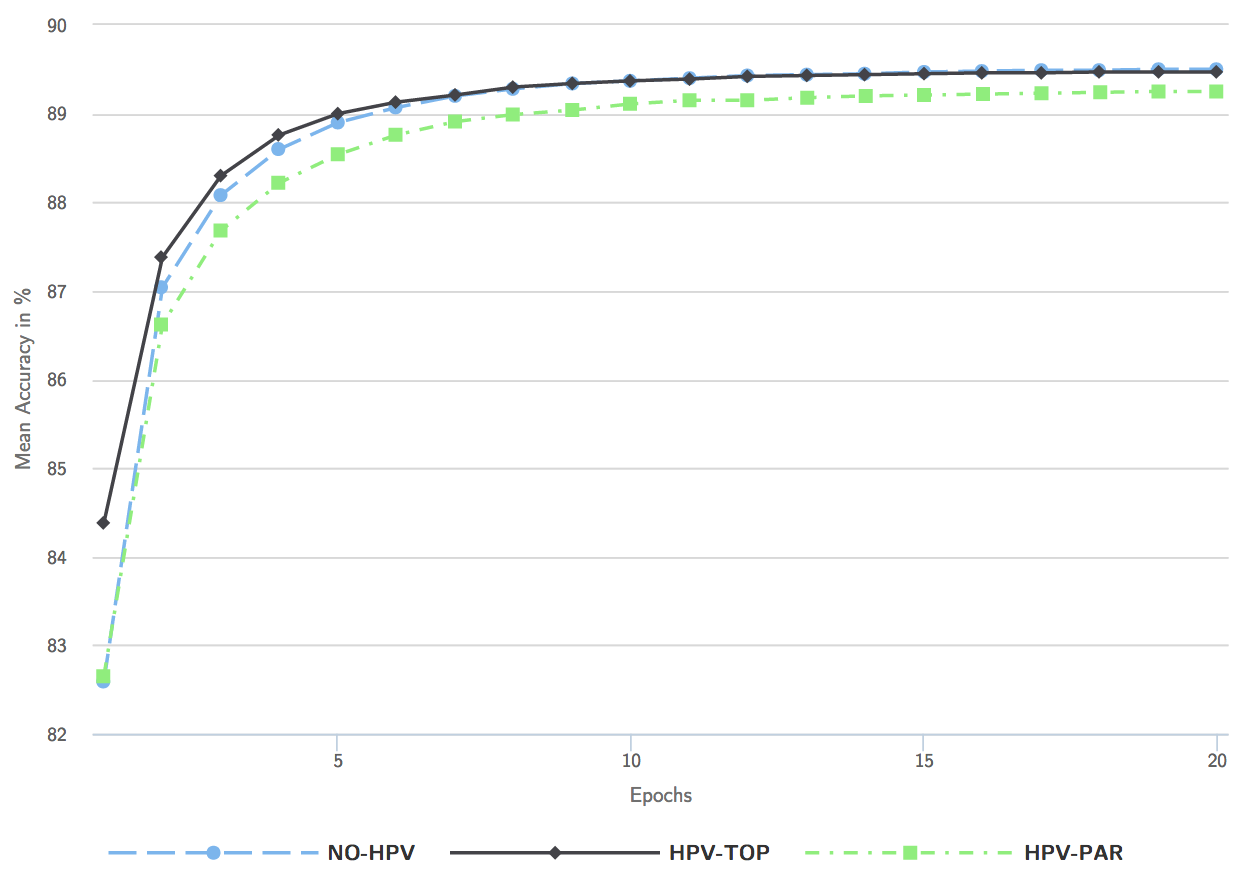
\includegraphics[width=1.0\textwidth]{5experiments/epochs-vs-accuracy-48.png}
	\caption{The mean accuracy of 30 experiments when increasing the epochs for the best configuration, using a word vector dimensionality of 48.}
	\label{fig:5:epochs-vs-accuracy-48}
\end{figure}

In Figure~\ref{fig:5:epochs-vs-accuracy-48} and Table~\ref{tab:5:epochs-vs-accuracy-48}, we again see an initial boost when using HPV-TOP compared to NO-HPV\@. However, after 8 epochs, the accuracy of HPV-TOP and NO-HPV converge. Also, in contrast to the 200 dimensional experiment, the accuracy increases slightly with further training.

For HPV-PAR, we notice similar behavior as before. After one epoch, the accuracy of HPV-PAR is the same as NO-HPV, and after that, HPV-PAR stays below NO-HPV and HPV-TOP\@.

\begin{table}
	\centering
	\caption{The data displayed in Figure~\ref{fig:5:epochs-vs-accuracy-48}, which is the restricted best configuration, using word vector dimensionality of 48. The values, where HPV-TOP outperforms NO-HPV with a level of significance of 0.025, are marked with a *. NO-HPV never outperforms HPV-TOP with a level of significance of 0.05 or lower.}
	\label{tab:5:epochs-vs-accuracy-48}
	\begin{tabular}{lrrr}
		\toprule
		& \multicolumn{3}{c}{\emph{Accuracy [\%]}}\tabularnewline
		\emph{Epoch}& \emph{HPV-NO}& \emph{HPV-TOP}& \emph{HPV-PAR}\tabularnewline
		\midrule
		1& 82.59& *84.38& 82.65\tabularnewline
		2& 87.04& *87.38& 86.62\tabularnewline
		3& 88.08& *88.3& 87.68\tabularnewline
		4& 88.6& *88.76& 88.22\tabularnewline
		5& 88.9& *89& 88.54\tabularnewline
		6& 89.07& *89.13& 88.76\tabularnewline
		7& 89.2& 89.21& 88.91\tabularnewline
		8& 89.28& 89.3& 88.99\tabularnewline
		9& 89.34& 89.34& 89.04\tabularnewline
		10& 89.37& 89.37& 89.11\tabularnewline
		11& 89.4& 89.39& 89.15\tabularnewline
		12& 89.43& 89.42& 89.15\tabularnewline
		13& 89.44& 89.43& 89.18\tabularnewline
		14& 89.45& 89.44& 89.2\tabularnewline
		15& 89.47& 89.45& 89.21\tabularnewline
		16& 89.48& 89.46& 89.22\tabularnewline
		17& 89.49& 89.46& 89.23\tabularnewline
		18& 89.49& 89.47& 89.24\tabularnewline
		19& 89.5& 89.47& 89.25\tabularnewline
		20& 89.5& 89.47& 89.25\tabularnewline
		\bottomrule
	\end{tabular}
\end{table}

\subsection{Execution Speed and Memory Usage}\label{5:execution-speed-and-memory-usage}

In this subsection, we compare the execution speed and the memory usage of the different HPV implementations. For the memory usage, we try to validate our theoretical calculation from~\ref{4:resources}.

\subsubsection{Execution Speed}

\begin{table}
	\centering
	\caption{Execution speed for training the word embeddings with a word vector dimensionality of 48 per epoch. 20 experiments per HPV implementation and model (HPV-DBOW, HPV-DM) have been conducted to calculate the average duration in seconds.}
	\label{tab:5:runtime48}
	\begin{tabular}{llrr}
		\toprule
		\emph{HPV}& \emph{Model}& \begin{tabular}[x]{@{}r@{}}\emph{Average}\\ \emph{Duration [s]}\end{tabular}& \begin{tabular}[x]{@{}r@{}}\emph{Standard}\\ \emph{Deviation}\end{tabular}\tabularnewline
		\midrule
		NO-HPV& HPV-DBOW& 23.71& 0.36\tabularnewline
		& HPV-DM& 18.01& 0.65\tabularnewline
		HPV-TOP& HPV-DBOW& 65.61& 0.61\tabularnewline
		& HPV-DM& 18.7& 0.42\tabularnewline
		HPV-TOP-PAR& HPV-DBOW& 88.85& 0.72\tabularnewline
		& HPV-DM& 27.2& 0.55\tabularnewline
		HPV-TOP-PAR-SENT& HPV-DBOW& 118.62& 9.19\tabularnewline
		& HPV-DM& 89.98& 4.3\tabularnewline
		HPV-PAR& HPV-DBOW& 45.91& 0.83\tabularnewline
		& HPV-DM& 26.98& 0.23\tabularnewline
		HPV-PAR-SENT& HPV-DBOW& 76.63& 3.56\tabularnewline
		& HPV-DM& 78.85& 0.22\tabularnewline
		HPV-PAR-SENT-SUBNV& HPV-DBOW& 111.79& 5.7\tabularnewline
		& HPV-DM& 135.13& 1.17\tabularnewline
		HPV-PAR-SENT-SUB& HPV-DBOW& 120.08& 2.84\tabularnewline
		& HPV-DM& 140.72& 1.6\tabularnewline
		\bottomrule
	\end{tabular}
\end{table}

To evaluate the execution speed, we ran 20 experiments with a word vector dimensionality of 48. The HPV implementation and the model influences the runtime substantially, which can be seen in Table \ref{tab:5:runtime48}. Furthermore, as we can see in Table \ref{tab:5:runtime48-totals}, in total, all HPV implementations are slower than the Doc2vec baseline. However, we notice that some [HPV, model] combinations, for example [NO-HPV, HPV-DM] or [HPV-TOP, HPV-DM], have comparable execution speed.

Overall, the advantage HPV gains by training ``faster'' compared to PV when using a fixed amount of epochs, it is overshadowed by the slower training speed of HPV per epoch. This effect is displayed in Figure~\ref{fig:5:epochs-vs-accuracy-200-scaled}, where the epochs are scaled according to the execution overhead.

\begin{figure}
	\centering
	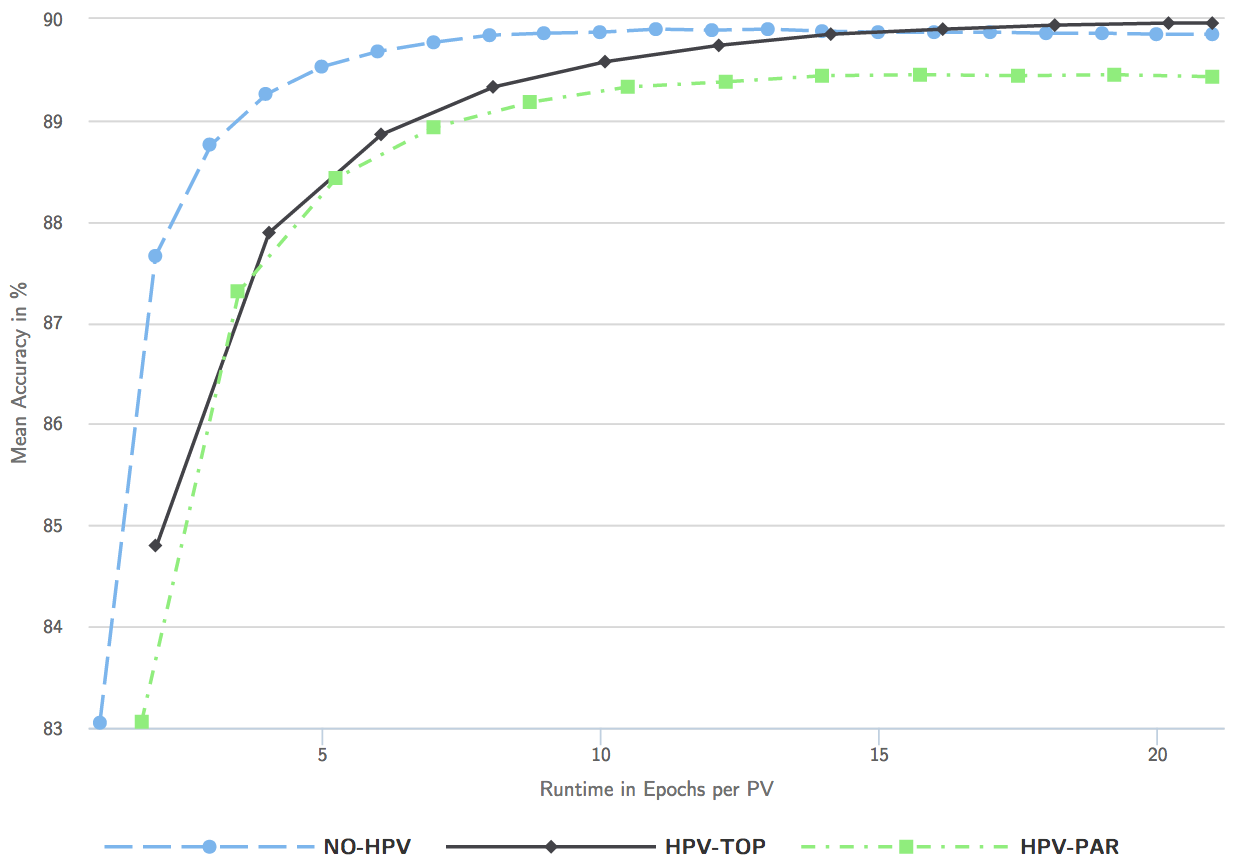
\includegraphics[width=1.0\textwidth]{5experiments/epochs-vs-accuracy-200-scaled.png}
	\caption{The mean accuracy of 30 experiments when increasing the epochs for the best configuration, using a word vector dimensionality of 200, where the epochs are scaled in relation to the execution overhead compared to NO-HPV. When considering this overhead, HPV-TOP trains considerably slower than NO-HPV, despite the initial boost in the first training epoch of HPV-TOP.}
	\label{fig:5:epochs-vs-accuracy-200-scaled}
\end{figure}

\begin{table}
	\centering
	\caption{Execution speed for training the word embeddings with a word vector dimensionality of 48 per epoch. Here, the results from Table \ref{tab:5:runtime48} are summarized.}
	\label{tab:5:runtime48-totals}
	\begin{tabular}{lrr}
		\toprule
		&  \multicolumn{2}{r}{\emph{Total Average Duration}}\tabularnewline
		\emph{HPV}& \emph{[s]} & \emph{[\%]}\tabularnewline
		\midrule
		NO-HPV& 41.72& 100\tabularnewline
		HPV-TOP& 84.31& 202\tabularnewline
		HPV-TOP-PAR& 116.05& 278\tabularnewline
		HPV-TOP-PAR-SENT& 208.60& 500\tabularnewline
		HPV-PAR& 72.89& 175\tabularnewline
		HPV-PAR-SENT& 155.48& 373\tabularnewline
		HPV-PAR-SENT-SUBNV& 246.92& 592\tabularnewline
		HPV-PAR-SENT-SUB& 260.80& 625\tabularnewline
		\bottomrule
	\end{tabular}
\end{table}


\subsubsection{Memory Usage}

Recall the formula for the additionally needed memory from \ref{4:resources}.
\begin{displaymath}
\frac{D \times G}{E \times \dim(U) +D \times K \times N}
\end{displaymath}

%todo low prio: add dim 200, add real memory

We ran the memory usage test with a window size $W=10$ and $D=E=48$ dimensions. From Table~\ref{tab:5:extracted-elements} we know $N=100'000$ documents, $Z=275$ average words per document, $dim(U)=185'957$ vocabulary size, and $K=1$ paragraph vectors per document. $G$ depends on the HPV implementation. From the results displayed in Table~\ref{tab:5:memory-usage} we notice that the formula for the memory usage overhead only fits approximately, and fails to predict the difference between HPV-PAR-SENT and HPV-PAR-SENT-SUBNV\@. At the time of writing, the source of this discrepancy is unknown, and may be caused by the implementation. Thus, it is not recommended to rely on the formula for the memory usage prediction.

\begin{table}
	\centering
	\caption{Predicted memory usage vs. measured memory usage, using a word vector dimensionality of 48. RAM is the measured ``real memory'' as reported by task\_info. It was measured during the training of the word embeddings model by using ``ps aux'' and represents a single observation.}
	\label{tab:5:memory-usage}
	\begin{tabular}{lrrrr}
		\toprule
		& & \multicolumn{3}{c}{\emph{Memory Overhead [\%]}} \tabularnewline
		& & \multicolumn{2}{c}{\emph{Serialized Model}} & \emph{RAM} \tabularnewline
		\emph{HPV}& \emph{$G$}& \emph{Predicted}& \emph{Measured}& \emph{Measured}\tabularnewline
		\midrule
		NO-HPV& 0& 0& 0& 0 \tabularnewline
		HPV-TOP& 20& 0& 0& 2 \tabularnewline
		HPV-TOP-PAR& 303468& 161& 121& 15 \tabularnewline
		HPV-TOP-PAR-SENT& 1916877& 1019& 780& 110 \tabularnewline
		HPV-PAR& 303448& 161& 121& 18 \tabularnewline
		HPV-PAR-SENT& 1916877& 1019& 780& 93 \tabularnewline
		HPV-PAR-SENT-SUBNV& 1916857& 1019& 1657& 120 \tabularnewline
		HPV-PAR-SENT-SUB& 4978237& 2647& 2039& 217 \tabularnewline
		\bottomrule
	\end{tabular}
\end{table}

%\begin{table}
%	\centering
%	\caption{toxxdo.}
%	\label{tab:xxxxxx}
%	\begin{tabular}{lr}
%		\toprule
%		\emph{AAA}& \emph{BBB}\tabularnewline
%		\midrule
%		XXX& YYY\tabularnewline
%		\bottomrule
%	\end{tabular}
%\end{table}

% \begin{tabular}[x]{@{}l@{}}TOP, PAR, SENT,\\SUB, SUBNV\end{tabular}























\chapter{Conclusion and Future Work}\label{conclusion-and-future-work}

To summarize, we introduced a novel method for generating high-quality low-dimensional word embeddings by extending the state-of-the-art methods PV-DM and PV-DBOW, using hierarchical data. We compared the novel algorithms HPV-DBOW and HPV-DM to the baselines PV-DM, PV-DBOW and TF-IDF\@.

We evaluated the word embeddings by applying HPV-DBOW and HPV-DM to the IMDB movie review dataset and measured the accuracy of the predicted sentiment. To retain comparable results, we conducted a broad search to find suitable hyperparameter combinations. We reached an accuracy of 90\%, using only elementary preprocessing.

Moreover, we implemented 7 different hierarchical paragraph vector variants, and conclude that using high-level hierarchies, such as topics and categories, we can increase the quality of the word embeddings at a cost of greater execution overhead. Low-level hierarchies, such as paragraphs and sentences, do not contribute to improving the quality of the word vectors. Furthermore, when using few training epochs, we have shown that hierarchical data can boost the quality of the word embeddings, but when scaled according to the execution speed, HPV trains slower than PV.

Finally, we analyzed the memory and runtime overhead when using HPV with different layers of hierarchies, and we compared it to PV-DM and PV-DBOW\@. While the overhead is significant, it is still feasible to process large amounts of text.

For future work, we suggest that HPV is evaluated on more datasets, where other hierarchies are available for training, and where HPV be evaluated on other tasks besides sentiment analysis. Furthermore, the embeddings should be trained and evaluated on larger corpora, so that multiple passes through the data may not be necessary.

Regarding the runtime and memory usage, we suggest that the implementation be analyzed in more detail. This can lead to optimizations which improve training speed and memory efficiency. Also, we recommend implementing different dimensionalities for word vectors and hierarchical paragraph vectors, ideally so that a different dimensionality can be defined per hierarchy layer.

Finally, more combinations of models and parameters should be evaluated, and HPV-DBOW and HPV-DM should be tested independently and in combination with other models.

%To summarize, we introduced a novel method to generate high-quality low-dimensionality word embeddings by extending the state of the art methods PV-DM and PV-DBOW to use hierarchical data. The newly introduced algorithms HPV-DBOW and HPV-DM have been shown to slightly outperform the baseline in sentiment analysis at a cost of greater overhead. Furthermore, we have shown that hierarchical data can boost the word embeddings quality when only few training epochs are used.
%We implemented 7 different hierarchical paragraph vector implementations, and we conclude that using high-level hierarchies, such as topics and categories, can increase the quality of the word embeddings, while low level hierarchies, such as paragraphs and sentences, do not contribute to improving the quality of the word vectors.
% Moreover, we evaluated the word embeddings quality by applying them to the IMDB dataset and predicting the sentiment for movie reviews. We reached an accuracy of 90\%, while using only elementary preprocessing. Moreover, we compared the novel method to the state of the art baselines PV-DM, PV-DBOW and TF-IDF\@.
% We conducted a broad search to find suitable hyperparameter combinations.


%\input{rules}
%\input{typography}
%\input{sections}

\appendix

\chapter{Appendix}

\section{Learning Rate Type}\label{appendix:learning-rate-type}

For all final experiments, a maximum learning rate of $l_{max}=0.025$ and a minimum learning rate of $l_{min}=0.001=10^{-3}$ have been used. In the beginning, we used $l_{min}=10^{-4}$, but after the learning rate decreased to below $10^{-3}$, the accuracy did not change anymore. Thus, the minimum learning rate was set to $10^{-3})$.

When only one epoch is scheduled, we use $l_{max}$. Otherwise, the learning rate is decreased after each epoch, using either a linear or an exponential function, see below.

\subsection{Linear}

By linear learning rate we mean a function which decreases linearly from the maximum learning rate $l_{max}$ to the minimum learning rate $l_{min}$. To calculate the learning rate for each step, we first set the learning rate of the first step to $l_{max}$, and the learning rate of the last step $n$ to $l_{min}$. The learning rate for epoch $i$ is calculated as follows.
\begin{displaymath}
l(i) = l_{max} - (i-1) \times \frac{l_{max} - l_{min}}{n-1}
\end{displaymath}

\subsection{Exponential}

The exponential case works analogously to the linear case. The learning rate for epoch $i$ is calculated as follows.
\begin{displaymath}
l(i) = l_{max} \times \left(\sqrt[l_{max}-1]{\frac{l_{min}}{l_{max}}}\right)^{i-1}
\end{displaymath}

%todo low prio: add graphs for the learning rate


\section{TF-IDF}\label{appendix:tf-idf}

We use scikit-learn version 0.16.1 for the TF-IDF calculation\footnote{\url{http://scikit-learn.org/stable/modules/generated/sklearn.feature_extraction.text.TfidfVectorizer.html}} with all default options, except the option ``max\_features'', which represents the maximum vector dimensionality.

From the documentation: ``The actual formula used for tf-idf is $tf \times (idf + 1) = tf + tf \times idf$, instead of $tf \times idf$. The effect of this is that terms with zero idf, i.e. that occur in all documents of a training set, will not be entirely ignored. [ \ldots ] Parameter max\_features: If not None, build a vocabulary that only consider the top max\_features features ordered by term frequency across the corpus.''

\section{Technical Implementation of Hierarchy Splitting}\label{appendix:hierarchy-splitting}

Hierarchy splitting is implemented in a modest fashion, which essentially works using regular expressions and is tuned towards the IMDB dataset. We use the following expressions to split each hierarchy. The implementation can be found here\footnote{\url{https://github.com/lukaselmer/hierarchical-paragraph-vectors}}.

\begin{description}
	\item[Paragraphs] ``\textless br /\textgreater \textless br /\textgreater'', ``\textless br /\textgreater'', ``\textless hr\textgreater''.
	\item[Sentences] ``!'', ``?'', ``.'', and consecutive combinations of these symbols, for example ``!!'' and ``!?!''.
	\item[Sub-sentences] ``,'', ``;'', ``:'', ``('', ``)''.
\end{description}

\backmatter

\bibliographystyle{plain}
\bibliography{refs}

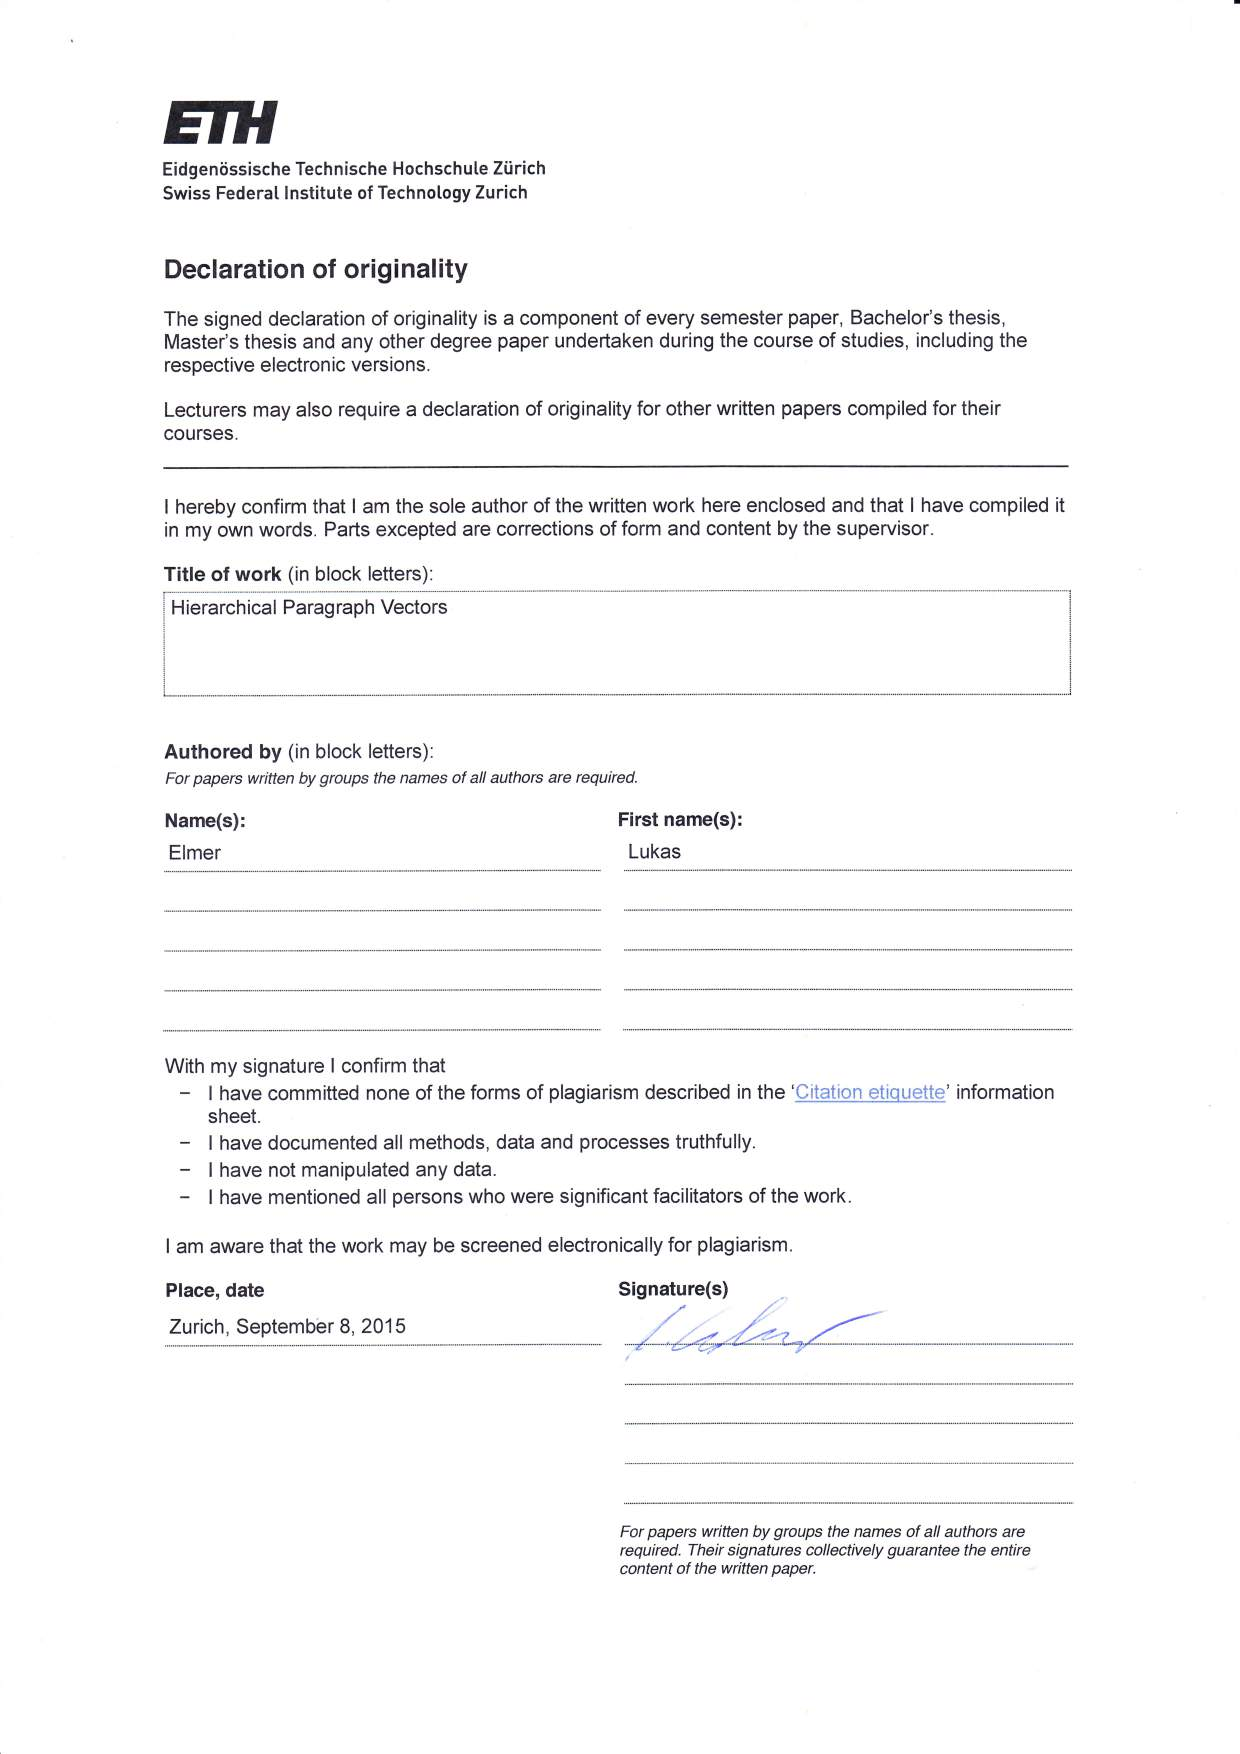
\includepdf[pages={-}]{0general/declaration-originality.pdf}

\end{document}

